% Paquets généraux
\documentclass[a4paper,12pt,titlepage,twoside]{article}
\usepackage[T1]{fontenc}
\usepackage[utf8]{inputenc}
\usepackage[french]{babel}
\usepackage{subcaption}
\addto\captionsfrench{%
  \renewcommand{\tablename}{Tableau}%
}
\usepackage[gen]{eurosym}
%\usepackage[dvips]{graphicx}
\usepackage{minted}
\usepackage{fancyhdr}
\usepackage{pdfpages} 
\usepackage{multido}
\usepackage{hyperref}
\usepackage{textcomp}
\usepackage{schemabloc}
%\usepackage[bitstream-charter]{mathdesign}
\usepackage{array}
\newcolumntype{P}[1]{>{\centering\arraybackslash}p{#1}}
\usepackage[shortlabels]{enumitem}
\usepackage[framemethod=TikZ]{mdframed}

\newcommand{\id}{71}
\newcommand{\nom}{Théorie des mécanismes}
\newcommand{\sequence}{04}
\newcommand{\nomsequence}{Liaisons entre les solides}
\newcommand{\num}{02}
\newcommand{\type}{KH}
\newcommand{\descrip}{Liaisons équivalentes, hyperstatisme, liaisons en série et en parallèle, théorie des graphes}
\newcommand{\competences}{B2-12: Proposer une modélisation des liaisons avec leurs caractéristiques géométriques. \\ &  B2-13: Proposer un modèle cinématique paramétré à partir d'un système réel, d'une maquette numérique ou d'u \\ &  B2-17: Simplifier un modèle de mécanisme. \\ &  B2-18: Modifier un modèle pour le rendre isostatique. \\ &  C1-04: Proposer une démarche permettant d'obtenir une loi entrée-sortie géométrique.  \\ &  C2-05: Caractériser le mouvement d'un repère par rapport à un autre repère. \\ &  C2-06: Déterminer les relations entre les grandeurs géométriques ou cinématiques. }
\newcommand{\nbcomp}{7}
\newcommand{\systemes}{}
\newcommand{\systemesnum}{}
\newcommand{\systemessansaccent}{}
\newcommand{\ilot}{2}
\newcommand{\ilotstr}{02}
\newcommand{\dossierilot}{\detokenize{Ilot_02 }}

%\usepackage{style}
\usepackage{bodegraph}
\usepackage{rpcinematik}
\usepackage[locale = FR]{siunitx}
\usepackage{caption}
\newcommand{\institute}{Lycée Dorian}

\usepackage{listings}
\usepackage{fancyvrb}
\usepackage{color}
\usepackage{xcolor}
\usepackage{colortbl}
\usepackage{helvet}
\usepackage[frenchmath]{newtxsf} % for sans serif symbols
\renewcommand{\familydefault}{\sfdefault}
%\usepackage{amsfonts}
%\usepackage{amsmath}
%\usepackage{lmodern}
\usepackage{mathastext}
%\usepackage{xspace}
\usepackage{varioref}
\usepackage{tabularx}
%\usepackage{floatflt}
\usepackage{graphics}
\usepackage{wrapfig}
\usepackage{textcomp}
\usepackage{tikz,tkz-tab}
\usepackage[european resistor, european voltage, european current]{circuitikz}
\usepackage{wrapfig}
\usepackage{gensymb}
\usepackage[percent]{overpic}
\usetikzlibrary{babel}
\usepackage{ifthen}
\usepackage{cancel}
\usepackage{etoolbox}
\usepackage{multirow}
%\usepackage{boxedminipage}
\definecolor{gris25}{gray}{0.75}
\definecolor{bleu}{RGB}{18,33,98}
\definecolor{bleuf}{RGB}{42,94,171}
\definecolor{bleuc}{RGB}{231,239,247}
\definecolor{bleum}{RGB}{160,195,226}
\definecolor{rougef}{RGB}{185,18,27}
\definecolor{rougec}{RGB}{255,188,204}%255,230,231
\definecolor{vertf}{RGB}{103,126,82}
\definecolor{vertc}{RGB}{220,255,191}
\definecolor{forestgreen}{rgb}{0.13,0.54,0.13}
\definecolor{blcr}{rgb}{0.59,0.69,0.84}
\definecolor{blfr}{rgb}{0.32,0.51,0.75}
\definecolor{orfr}{rgb}{0.90,0.42,0.15}
\definecolor{orcr}{rgb}{0.90,0.65,0.50}
\definecolor{orangef}{rgb}{0.659,0.269,0.072}
\definecolor{orange}{rgb}{0.58,0.35,0.063}
\definecolor{orangec}{rgb}{0.43,0.32,0.25}
\definecolor{rcorrect}{rgb}{0.6,0,0}
\definecolor{sequence}{rgb}{0.75,0.75,0.75}
\definecolor{competences}{rgb}{0.61,0.73,0.35}
\definecolor{rose}{HTML}{ff00ff}
\definecolor{grisf}{HTML}{222222}
\definecolor{grisc}{HTML}{636363}
\definecolor{normal}{HTML}{4087c4}
\definecolor{info}{HTML}{5bc0de}
\definecolor{success}{RGB}{92,184,92}
\definecolor{warning}{RGB}{240,173,78}
\definecolor{danger}{RGB}{217,83,79}
\hypersetup{                    % parametrage des hyperliens
    colorlinks=true,                % colorise les liens
    breaklinks=true,                % permet les retours à la ligne pour les liens trop longs
    urlcolor= blfr,                 % couleur des hyperliens
    linkcolor= orange,                % couleur des liens internes aux documents (index, figures, tableaux, equations,...)
    citecolor= forestgreen                % couleur des liens vers les references bibliographiques
    }

\newcolumntype{M}[1]{>{\centering\arraybackslash}m{#1}}
\definecolor{codegreen}{rgb}{0,0.6,0}
\definecolor{codegray}{rgb}{0.5,0.5,0.5}
\definecolor{codepurple}{rgb}{0.58,0,0.82}
\definecolor{backcolour}{rgb}{0.95,0.95,0.92}

\lstdefinestyle{mystyle}{
    backgroundcolor=\color{backcolour},   
    commentstyle=\color{codegreen},
    keywordstyle=\color{magenta},
    numberstyle=\tiny\color{codegray},
    stringstyle=\color{codepurple},
    basicstyle=\ttfamily\footnotesize,
    breakatwhitespace=false,         
    breaklines=true,                 
    captionpos=b,                    
    keepspaces=true,                 
    numbers=left,                    
    numbersep=5pt,                  
    showspaces=false,                
    showstringspaces=false,
    showtabs=false,                  
    tabsize=2
}

\lstset{style=mystyle}

% Mise en page
\pagestyle{fancy}

\setlength{\hoffset}{-18pt}
\setlength{\oddsidemargin}{0pt} 	% Marge gauche sur pages impaire2s
\setlength{\evensidemargin}{0pt} 	% Marge gauche sur pages paires
\setlength{\marginparwidth}{00pt} 	% Largeur de note dans la marge
\setlength{\headwidth}{481pt} 	 	% Largeur de la zone de tête (17cm)
\setlength{\textwidth}{481pt} 	 	% Largeu\textbf{r de la zone de texte (17cm)
\setlength{\voffset}{-18pt} 		% Bon pour DOS
\setlength{\marginparsep}{7pt}	 	% Séparation de la marge
\setlength{\topmargin}{-30pt} 		% Pas de marge en haut
\setlength{\headheight}{55pt} 		% Haut de page
\setlength{\headsep}{20pt} 		% Entre le haut de page et le texte
\setlength{\footskip}{30pt} 		% Bas de\textbf{ page + séparation
\setlength{\textheight}{700pt} 		% Hauteur de l'icone zone de texte (25cm)
\setlength\fboxrule{1 pt}
\renewcommand{\baselinestretch}{1}
\setcounter{tocdepth}{1}
\newcommand{\cadre}[2]
{\fbox{
  \begin{minipage}{#1\linewidth}
   \begin{center}
    #2\\
   \end{center}
  \end{minipage}
 }
}

\newcommand{\repon}[1]
{
~\ \\
\begin{tabular}{|m{\linewidth}|}
 \hline
\multido{}{#1}{\\ \hline}
\end{tabular}
}


\newcommand{\objectif}[1]{
\mdfsetup{%
frametitle={%
\tikz[baseline=(current bounding box.east),outer sep=0pt]
\node[anchor=east,rectangle,fill=bleum]
{\strut Objectif~};}}
\mdfsetup{innertopmargin=10pt,linecolor=bleum,%
linewidth=2pt,topline=true,%
frametitleaboveskip=\dimexpr-\ht\strutbox\relax
}
\begin{mdframed}[]\relax%
#1
\end{mdframed}}


\newcounter{num_quest} \setcounter{num_quest}{0}
\newcounter{num_rep} \setcounter{num_rep}{0}
\newcounter{num_cor} \setcounter{num_cor}{0}

\newcommand{\feuilleDR}[1]{
	\begin{tikzpicture}
		\draw[gray!30](0,0)grid[step=0.5cm](\linewidth,#1);
	\end{tikzpicture}
}

%\newcommand{\question}[1]{\refstepcounter{num_quest}\par
%~\ \\ \parbox[t][][t]{0.15\linewidth}{\textbf{Question \arabic{num_quest}}}\parbox[t][][t]{0.85\linewidth}{#1\label{q\the\value{num_quest}}}\par
%}

\newcommand{\question}[1]{\refstepcounter{num_quest}\par
~\ \\ \textbf{Question \arabic{num_quest} : }#1\label{q\the\value{num_quest}}\par
}

\newcommand{\posetafigure}[3]{
\begin{figure}[ht!]
 \begin{center}
  \includegraphics[width=#2\linewidth]{img/#1}
 \end{center}
 \caption{\label{#1} #3}
\end{figure}}

\newcommand{\goforum}{
\begin{figure}

\end{figure}
\begin{center}
 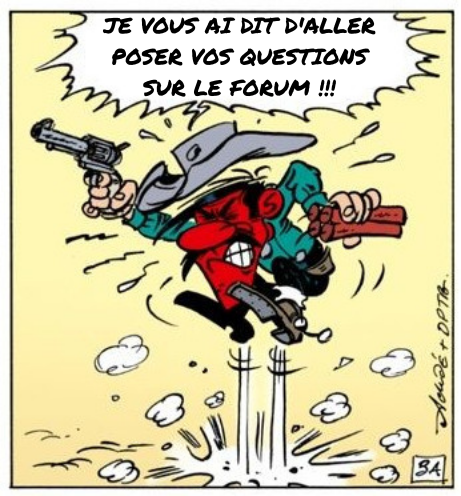
\includegraphics[width=0.7\linewidth]{../../../img/go_forum}
\end{center}
\label{go_forum}
\caption{J'pète les plombs}
\end{figure}}

\newcommand{\reponse}[4][1]
{\noindent
\parbox{\textwidth}{
\rule{\linewidth}{.5pt}\\
\textbf{Question\ifthenelse{#1>1}{s}{} \multido{}{#1}{%
\refstepcounter{num_rep}\ref{q\the\value{num_rep}} }:} ~\ \\
\ifdef{\public}{#3 \ifthenelse{#2>0}{~\ \\ 	\feuilleDR{#2}}}{#4}
}}

\newcommand{\cor}
{\refstepcounter{num_cor}
\noindent
\rule{\linewidth}{.5pt}
\textbf{Question \arabic{num_cor}:} \\
}

\newcommand{\finsujet}
{
    \begin{center}
    \Large{FIN}
    \end{center}

    \cleardoublepage

    \ifdef{\public}{\pagestyle{docreponse}}{\pagestyle{correction}}

    \ifdef{\public}{
        \begin{tikzpicture} 
            \draw (0,0) rectangle (2,2);
            \draw (0,0) -- (2,2);
            \draw (1.5,0.5) node {\large 20};
            \draw (2.5,0) rectangle (16,2);
            \draw (4.5,1.7) node {\large Commentaires:};
        \end{tikzpicture}
    }
    ~\ \\
}


%\newcommand{\repcarre}[2]
%{
%~\ \\
%\begin{tikzpicture}
%\draw [fill=white] (0,0) rectangle +(\linewidth,#1);
%\node[align=left] at (1.1,#2-0.3) {\textbf{Question #1:}};
%\end{tikzpicture}
%}

\newcommand{\titre}[1]
{\begin{center}
\cadre{0.8}{\huge #1} 
\end{center}
}


%Définition des torseurs :
\newcommand{\torseur}[2]{\left\{\mathcal{#1}_{#2} \right\}}
\newcommand{\torseurh}[3]{\left\{\genfrac{}{}{0pt}{0}{#1}{#2}\right\}_{#3}}
\newcommand{\torseurv}[8]{\left\{
\begin{matrix}
#1 & #4 \\ #2 & #5 \\ #3 &#6
\end{matrix}
\right\}_{{#7},{#8}}}

%Définition des torseurs :
%\newcommand{\torseur}[2]{\left \{\mbox{\relsize{2}{$\mathcal {#1}$}\relsize{-2}}\phantom{}_{\mbox{\scriptsize $#2$}} \right \}}
%\newcommand{\torseurh}[3]{\left\{\genfrac{}{}{0pt}{0}{#1}{#2}\right\}_{#3}}
%\newcommand{\torseurv}[8]{
%\left\{\begin{array}{@{}c|c@{}} #1 & #4 \\ #2 & #5 \\ #3 & #6 \end{array} \right\}_{#7,#8}
%}
\newcommand{\derivee}[2]{\left.\dfrac{\d #1}{\d t}\right|_{#2}}
\newcommand{\tripleint}{\int\!\!\!\!\!\int\!\!\!\!\!\int}

% Notation cinématique et statique
\newcommand{\cinematique}[2]{\mbox{#1}/\mbox{#2}}
\newcommand{\statique}[2]{\mbox{#1}\rightarrow\mbox{#2}}
\newcommand{\moment}[3]{\vv {#1}_{\scriptsize{#3}}(#2)}
\newcommand{\resultante}[2]{\vv {#1}_{\scriptsize{#2}}}


%Commande de base
\newcommand{\jo}{\left(j\omega\right)} % j \omega dans l'analyse fréquentielle
\newcommand{\tl}{\xrightarrow{\mathcal{L}}} % transformée de laplace sur fleche
\newcommand{\tli}{\xrightarrow{\mathcal{L}^{-1}}} % transformée inverse de laplace sur fleche
\renewcommand{\d}[1][]{\mathrm{d#1}}
\newcommand{\dd}[1][]{\mathrm{d#1}}
\newcommand{\vect}[2]{{#1}\wedge{#2}}
\newcommand{\base}[3]{(\vec #1,\vec #2,\vec #3)}
\newcommand{\vectbase}[4]{{\vphantom{\left| \begin{matrix}
#1\\#2\\#3 \end{matrix} \right|}}_{#4}{\left| \begin{matrix}
#1\\#2\\#3 \end{matrix} \right.}}
%Pour avoir les paragraphes sous la forme I, II, III
\renewcommand{\thesection}{\Roman{section}}
\setcounter{secnumdepth}{3}
\renewcommand{\Frlabelitemii}{$\bullet$}

% En tête et pied de page
\lhead{\nom}
\rhead{
\includegraphics[width=2cm]{../../../img/logo}}
\lfoot{\auteurun,\ \auteurdeux}
\cfoot{Page \thepage}

\fancypagestyle{docreponse}{%
  \fancyhf{}
  \fancyhead[LO]{NOM Prénom: .............................}
  \rhead{
\includegraphics[width=2cm]{../../../img/logo}\hspace{2pt}}
  \ifdef{\auteurdeux}{\lfoot{\auteurun,\ \auteurdeux}}{\lfoot{\auteurun}}
  \rfoot{\nom}
  \lfoot{Document réponse}
  \cfoot{Page \thepage}
   }

\fancypagestyle{correction}{%
  \fancyhf{}
  \lhead{\colorbox{danger}{\begin{minipage}{0.65\paperwidth} \textcolor{white}{\textbf{Correction}} \end{minipage}} }
  \rhead{
\includegraphics[width=2cm]{../../../img/logo}}
  \lfoot{Renaud Costadoat, Françoise Puig}
  \rfoot{\colorbox{danger}{\begin{minipage}{0.4\paperwidth} \begin{flushright}\textcolor{white}{\textbf{Correction}}\end{flushright} \end{minipage}} }}

\fancypagestyle{correctioninfo}{%
  \fancyhf{}
  \lhead{\colorbox{danger}{\begin{minipage}{0.65\paperwidth} \textcolor{white}{\textbf{Correction}} \end{minipage}} }
  \rhead{
\includegraphics[width=2cm]{../../../img/logo}}
  \lfoot{Renaud Costadoat, Juliette Genzmer}
  \rfoot{\colorbox{danger}{\begin{minipage}{0.6\paperwidth} \begin{flushright}\textcolor{white}{\textbf{Correction}}\end{flushright} \end{minipage}} }}

\renewcommand{\footrulewidth}{0.4pt}

\usepackage{eso-pic}
\newcommand{\BackgroundPic}{%
\put(0,0){%
\parbox[b][\paperheight]{\paperwidth}{%
\vfill
\begin{center}
\hspace{0.5cm}\vspace{0.5cm}

\includegraphics[width=\paperwidth,height=\paperheight,%
keepaspectratio]{../../../img/fond3}%
\end{center}
\vfill
}}}

\newcommand{\BackgroundPicdeux}{%
\put(25,-30){%
\parbox[b][\paperheight]{\paperwidth}{%
\vfill
\begin{center}
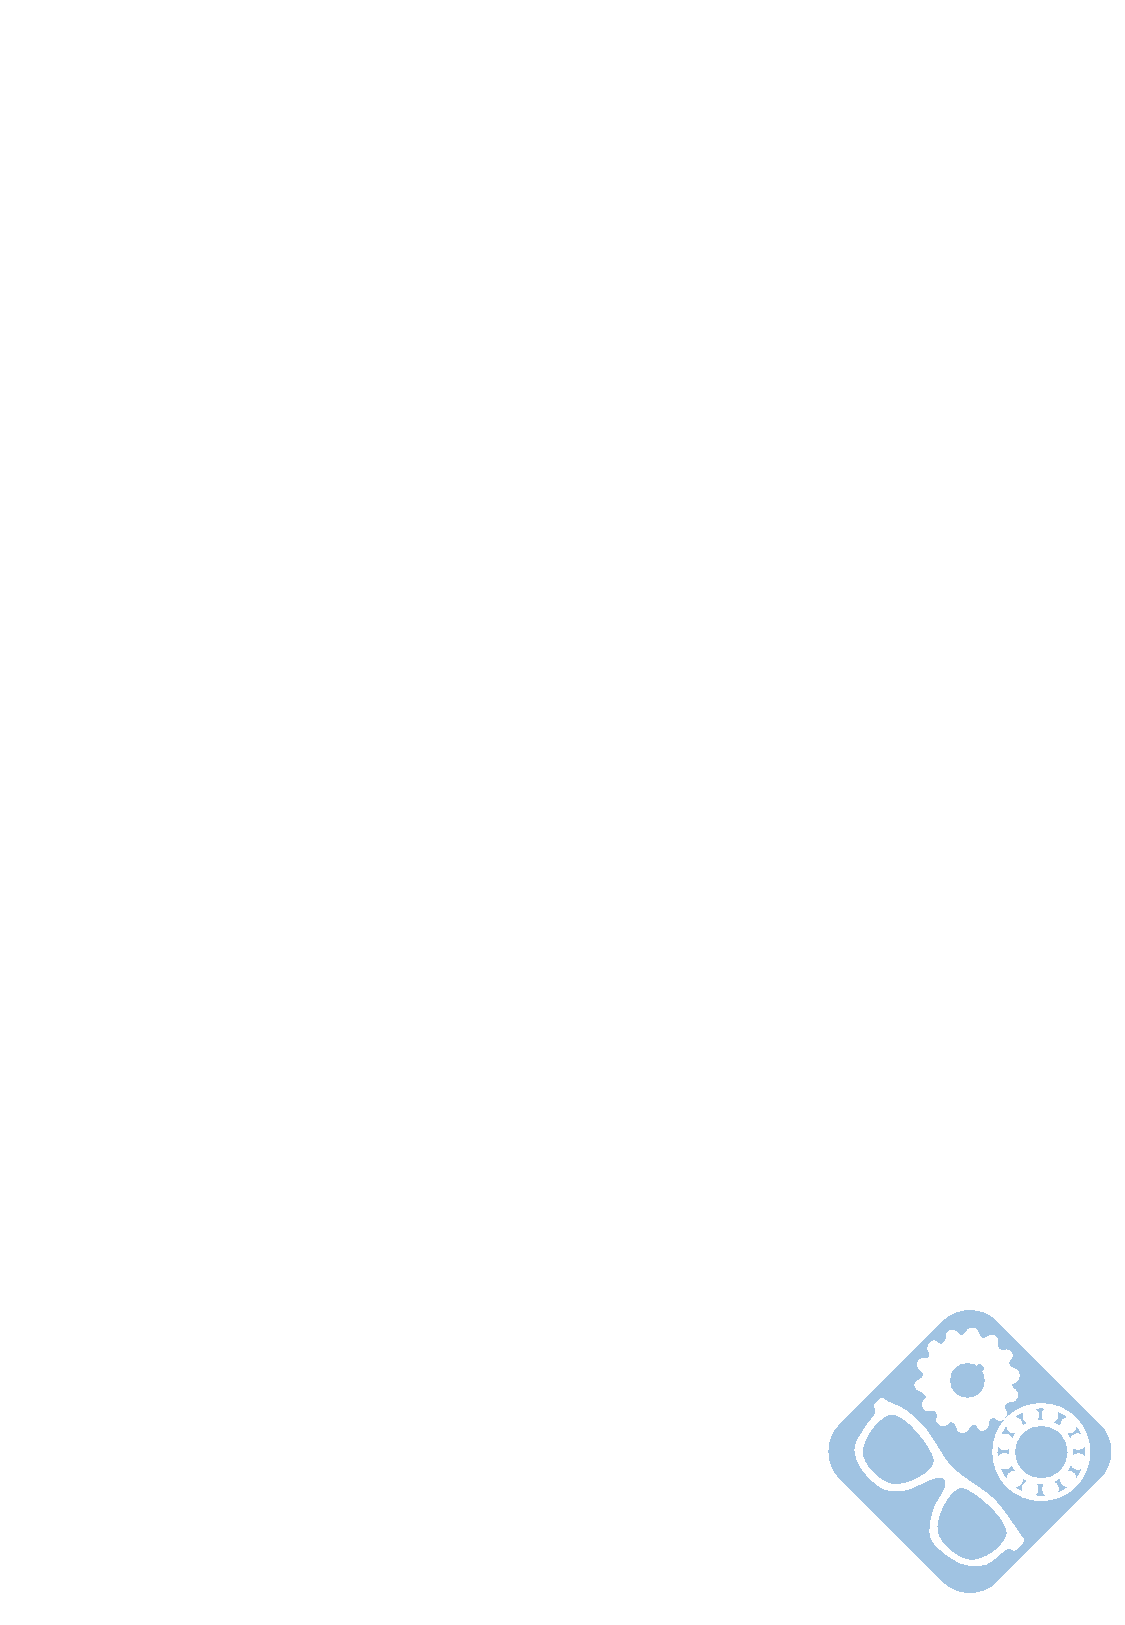
\includegraphics[width=\paperwidth,height=\paperheight,%
keepaspectratio]{../../../img/fond4}%
\end{center}
\vfill
}}}

\begin{document}

\pagestyle{empty}

\AddToShipoutPicture*{\BackgroundPic}


\includegraphics[width=2cm]{../../../img/logo}

\Huge{DS \numero - \sujet}

\vspace{1cm}

\ifdef{\prive}{\begin{center}\colorbox{danger}{\Huge{Avec Correction}}\end{center}}{}

\begin{center}
\centering\huge{PTSI}
\end{center}

\vspace{2cm}


\begin{center}
\centering\Large{\jour}
\end{center}

\vspace{2cm}

\normalsize

\tableofcontents

\newpage

\AddToShipoutPicture{\BackgroundPicdeux}

\pagestyle{fancy}

\begin{center}
\Huge \sujet
\end{center}


\normalsize


\section{Présentation générale (30 min)}

\subsection{Introduction}

Les constructeurs automobiles sont sans cesse dans l'obligation d'innover pour rester attractifs vis-à-vis du client. Les ouvrants pilotés automobiles font partie des atouts différenciateurs. Le terme ouvrant désigne à la fois les lève-vitres électriques, les toits ouvrants, les toits escamotables, les coffres motorisés et les portes latérales coulissantes. Tous ces ouvrants sont une source d'attrait pour le client, de par leur praticité ou encore par leurs facteurs de différenciation importants.

\begin{figure}[!h]
 \centering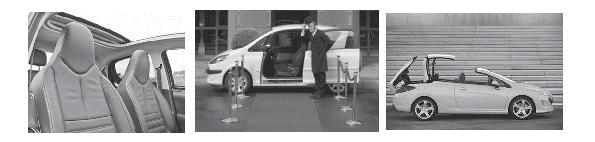
\includegraphics[width=0.9\linewidth]{img/img01}
 \caption{Différents types d'ouvrants du groupe PSA}
 \label{img01}
\end{figure}

Il existe deux types de pilotage des ouvrants :
\begin{itemize}
 \item le premier est un système classique et/ou d'assistance. L'utilisateur gère complètement le déplacement de l'ouvrant. Dès qu'il arrête son action sur la commande, l'ouvrant s'immobilise, c'est le cas par exemple du lève-vitre électrique non séquentiel. Ainsi, avec un système classique et/ou d'assistance, le déplacement de l'ouvrant est entièrement imputable aux actions de l'utilisateur,
 \item le second type est le pilotage automatisé des ouvrants. Ici, l'utilisateur demande simplement à ce que l'ouvrant se déplace jusqu'à une position prédéfinie. Une brève action de sa part entraîne le déplacement complet de l'ouvrant. Pour le lève-vitre électrique séquentiel, l'utilisateur demande à ce que la vitre remonte complètement, par une courte action sur l'interrupteur. Dès lors, le système de contrôle/commande gère le déplacement de l'ouvrant dans le cas normal, mais aussi en cas de dysfonctionnement (perte de fonctionnalité ou présence d'un obstacle sur le trajet de la vitre). Il faut donc assurer un fonctionnement sûr et robuste du système d'ouvrant piloté automatisé pour éviter que le système blesse un occupant.
\end{itemize}

Le diagramme de cas d'utilisation de la figure \ref{img02} synthétise les explications précédentes.

\newpage

\begin{figure}[!h]
 \centering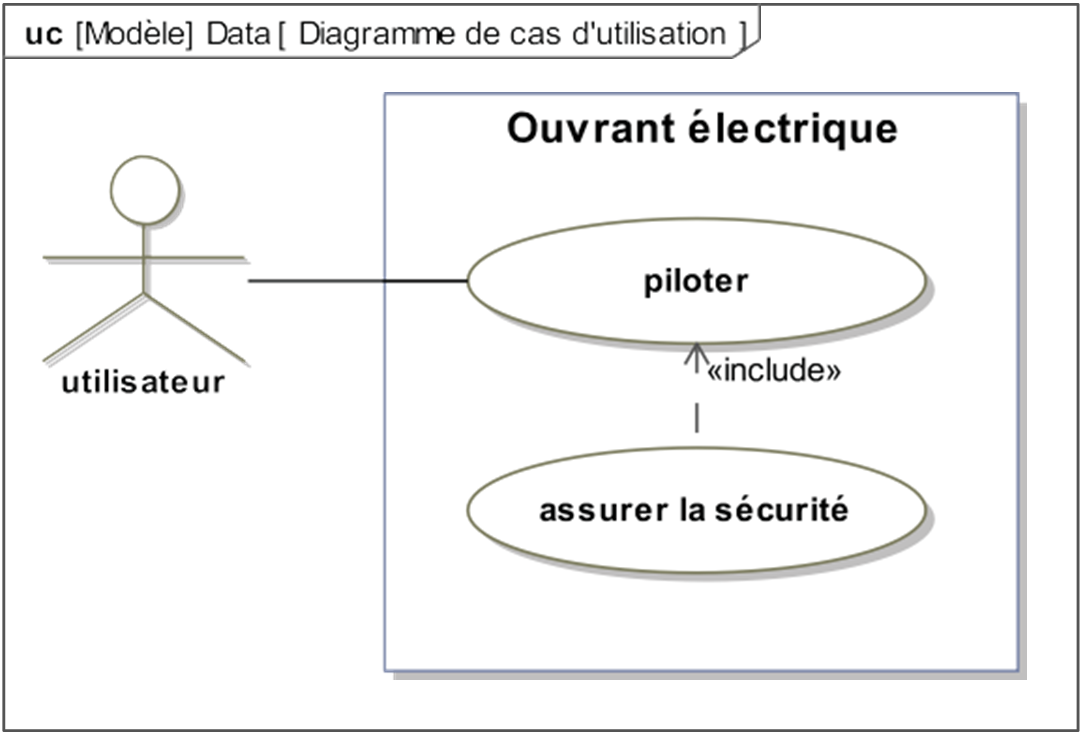
\includegraphics[width=0.5\linewidth]{img/img02}
 \caption{Diagramme de cas d'utilisation d'un ouvrant électrique}
 \label{img02}
\end{figure}

Objectif:

L'objectif du travail proposé dans ce sujet est de mettre en place différentes stratégies de commande d'un lève-vitre électrique de Peugeot 308 de manière à pouvoir extrapoler les résultats à une porte coulissante électrique.

~\

Cette étude nécessite :
\begin{itemize}
 \item une analyse de l'architecture du lève-vitre (partie I),
 \item une modélisation multiphysique du système (partie II),
 \item la mise en place d'un modèle de commande tout ou rien (partie III),
 \item le développement d'un modèle de commande de type asservissement continu (partie IV). Le diagramme des exigences de la figure \ref{img03} liste quelques performances attendues pour le lève-vitre électrique.
\end{itemize}

\begin{figure}[!h]
 \centering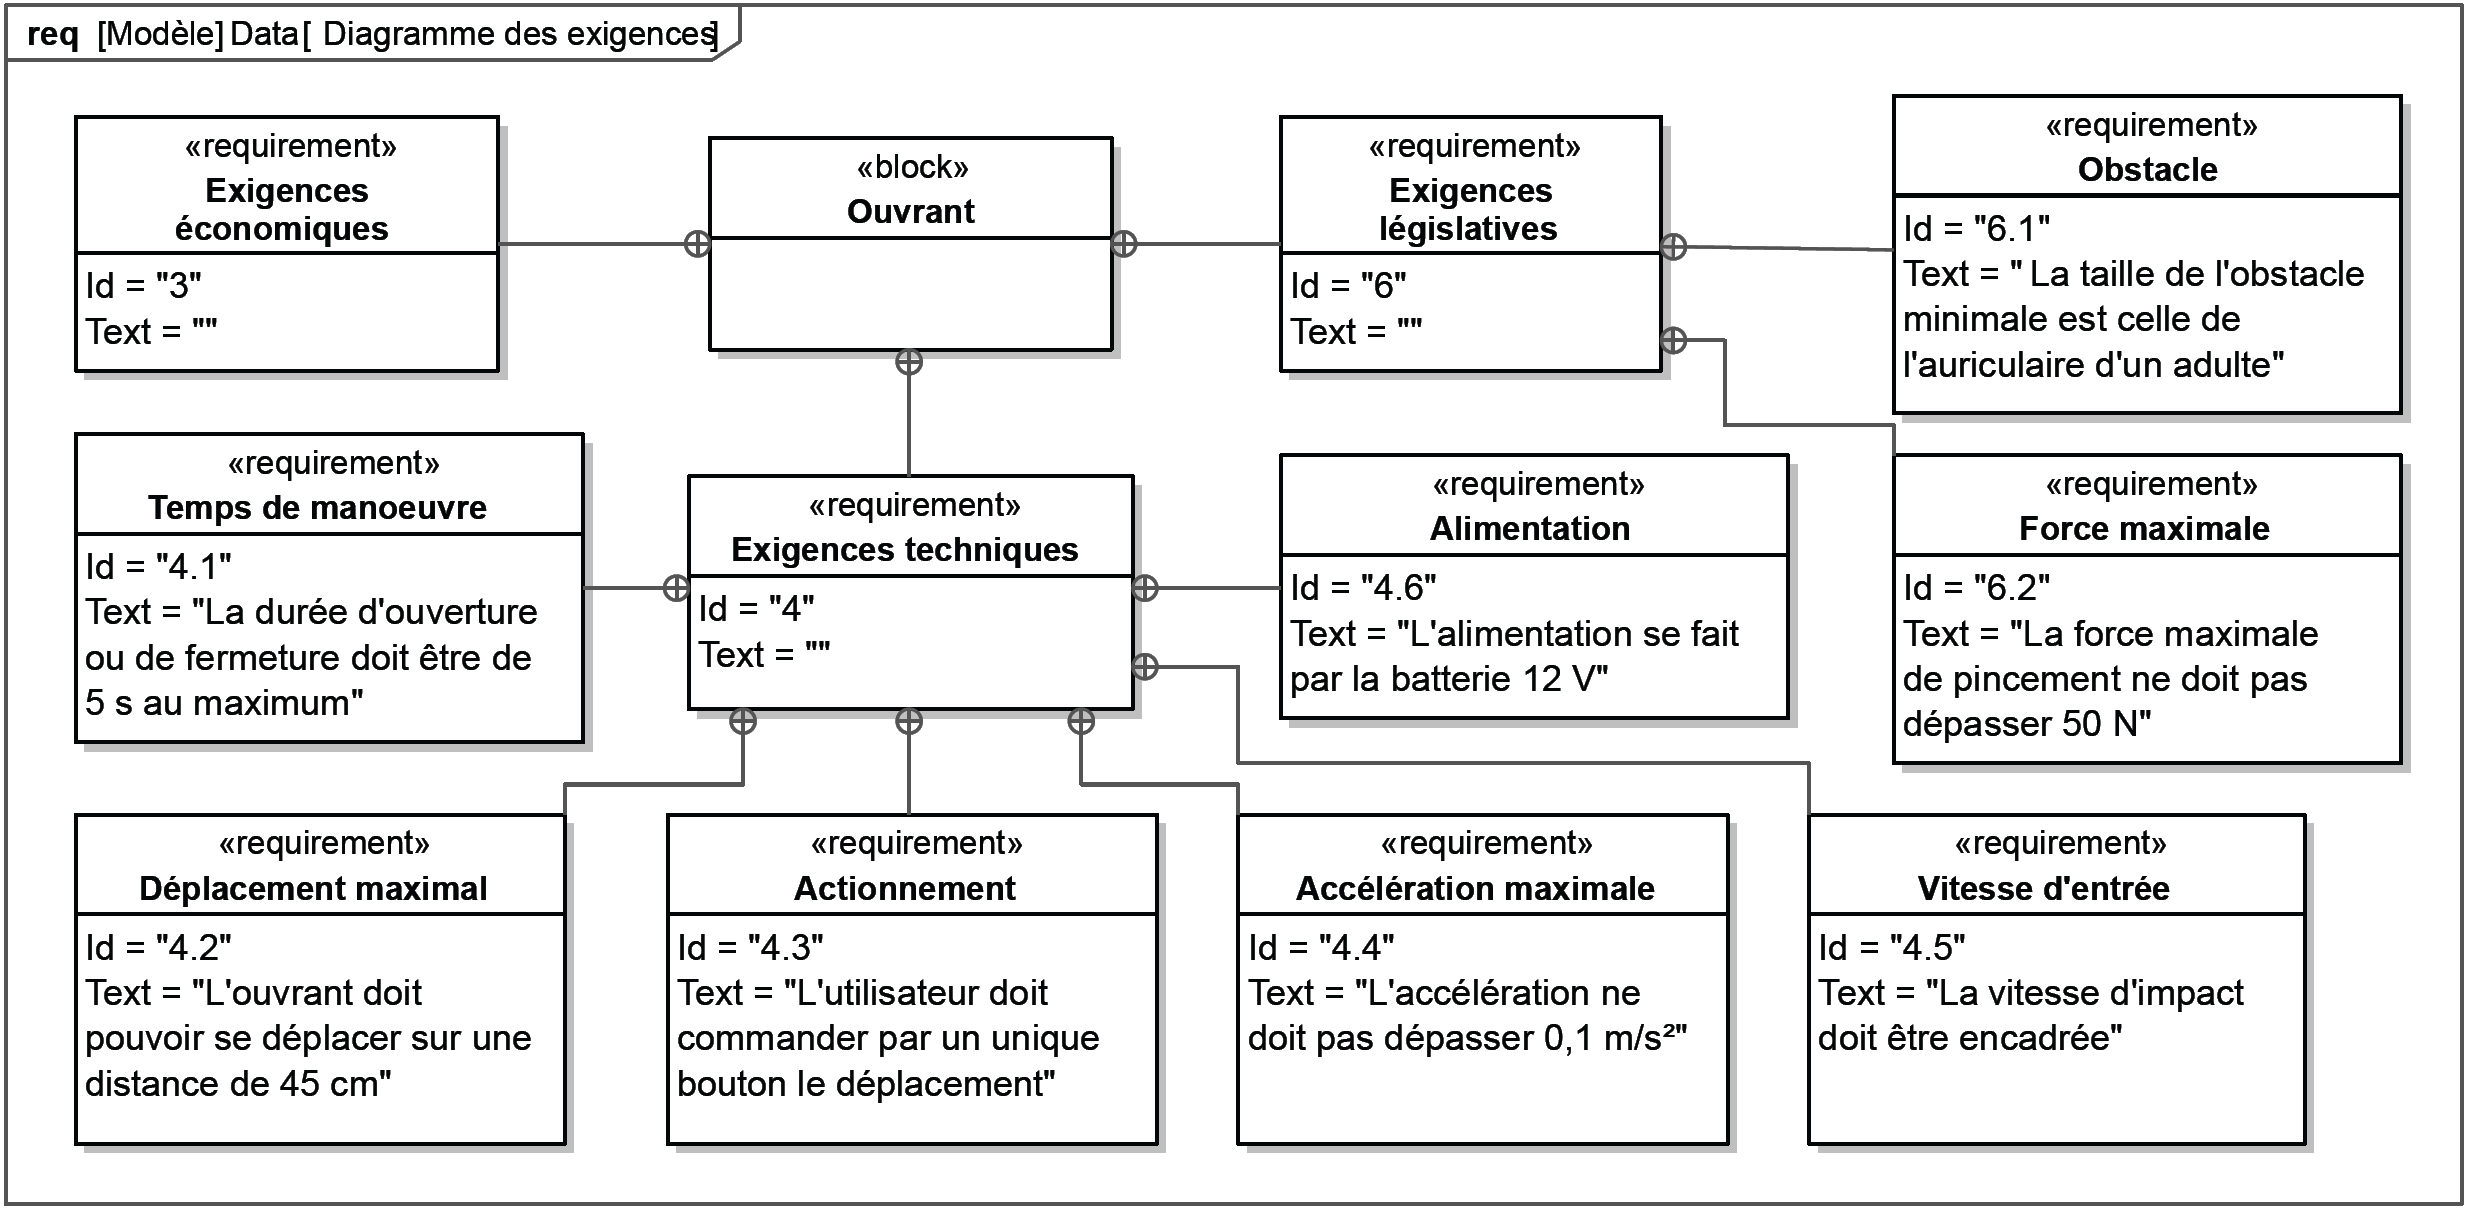
\includegraphics[width=0.9\linewidth]{img/img03}
 \caption{Diagramme des exigences}
 \label{img03}
\end{figure}

\section{Architecture du lève-vitre}

Pour le développement et la mise en \oe uvre d'une architecture de commande, il est nécessaire de disposer d'un modèle de simulation fiable et précis, tout en connaissant ses limites de validité. L'élaboration d'un tel modèle nécessite de décrire l'implantation de la chaîne d'énergie et de la chaîne d'informations de l'ouvrant.

Le diagramme de définitions de blocs de la figure \ref{img04}, liste l'ensemble des constituants principaux du lève-vitre électrique. La plupart des constituants sont repérés sur les vues tridimensionnelles données en annexe figures \ref{an01}, \ref{an011} et \ref{an02}.

\paragraph{Question 1:} Compléter, à l'aide des noms disponibles sur le diagramme de la figure \ref{img04}, le schéma des chaînes fonctionnelles du document réponse.

~\

Le réducteur du lève-vitre est constitué d'un dispositif roue et vis sans fin. La roue possède $Z=53$ dents et la vis est constituée d'un filet. Le câble s'enroule sur le tambour de diamètre $D=41,5mm$, solidaire de la roue. Le câble est solidaire du coulisseau sur lequel est fixée la vitre.
 
\begin{figure}[!h]
 \centering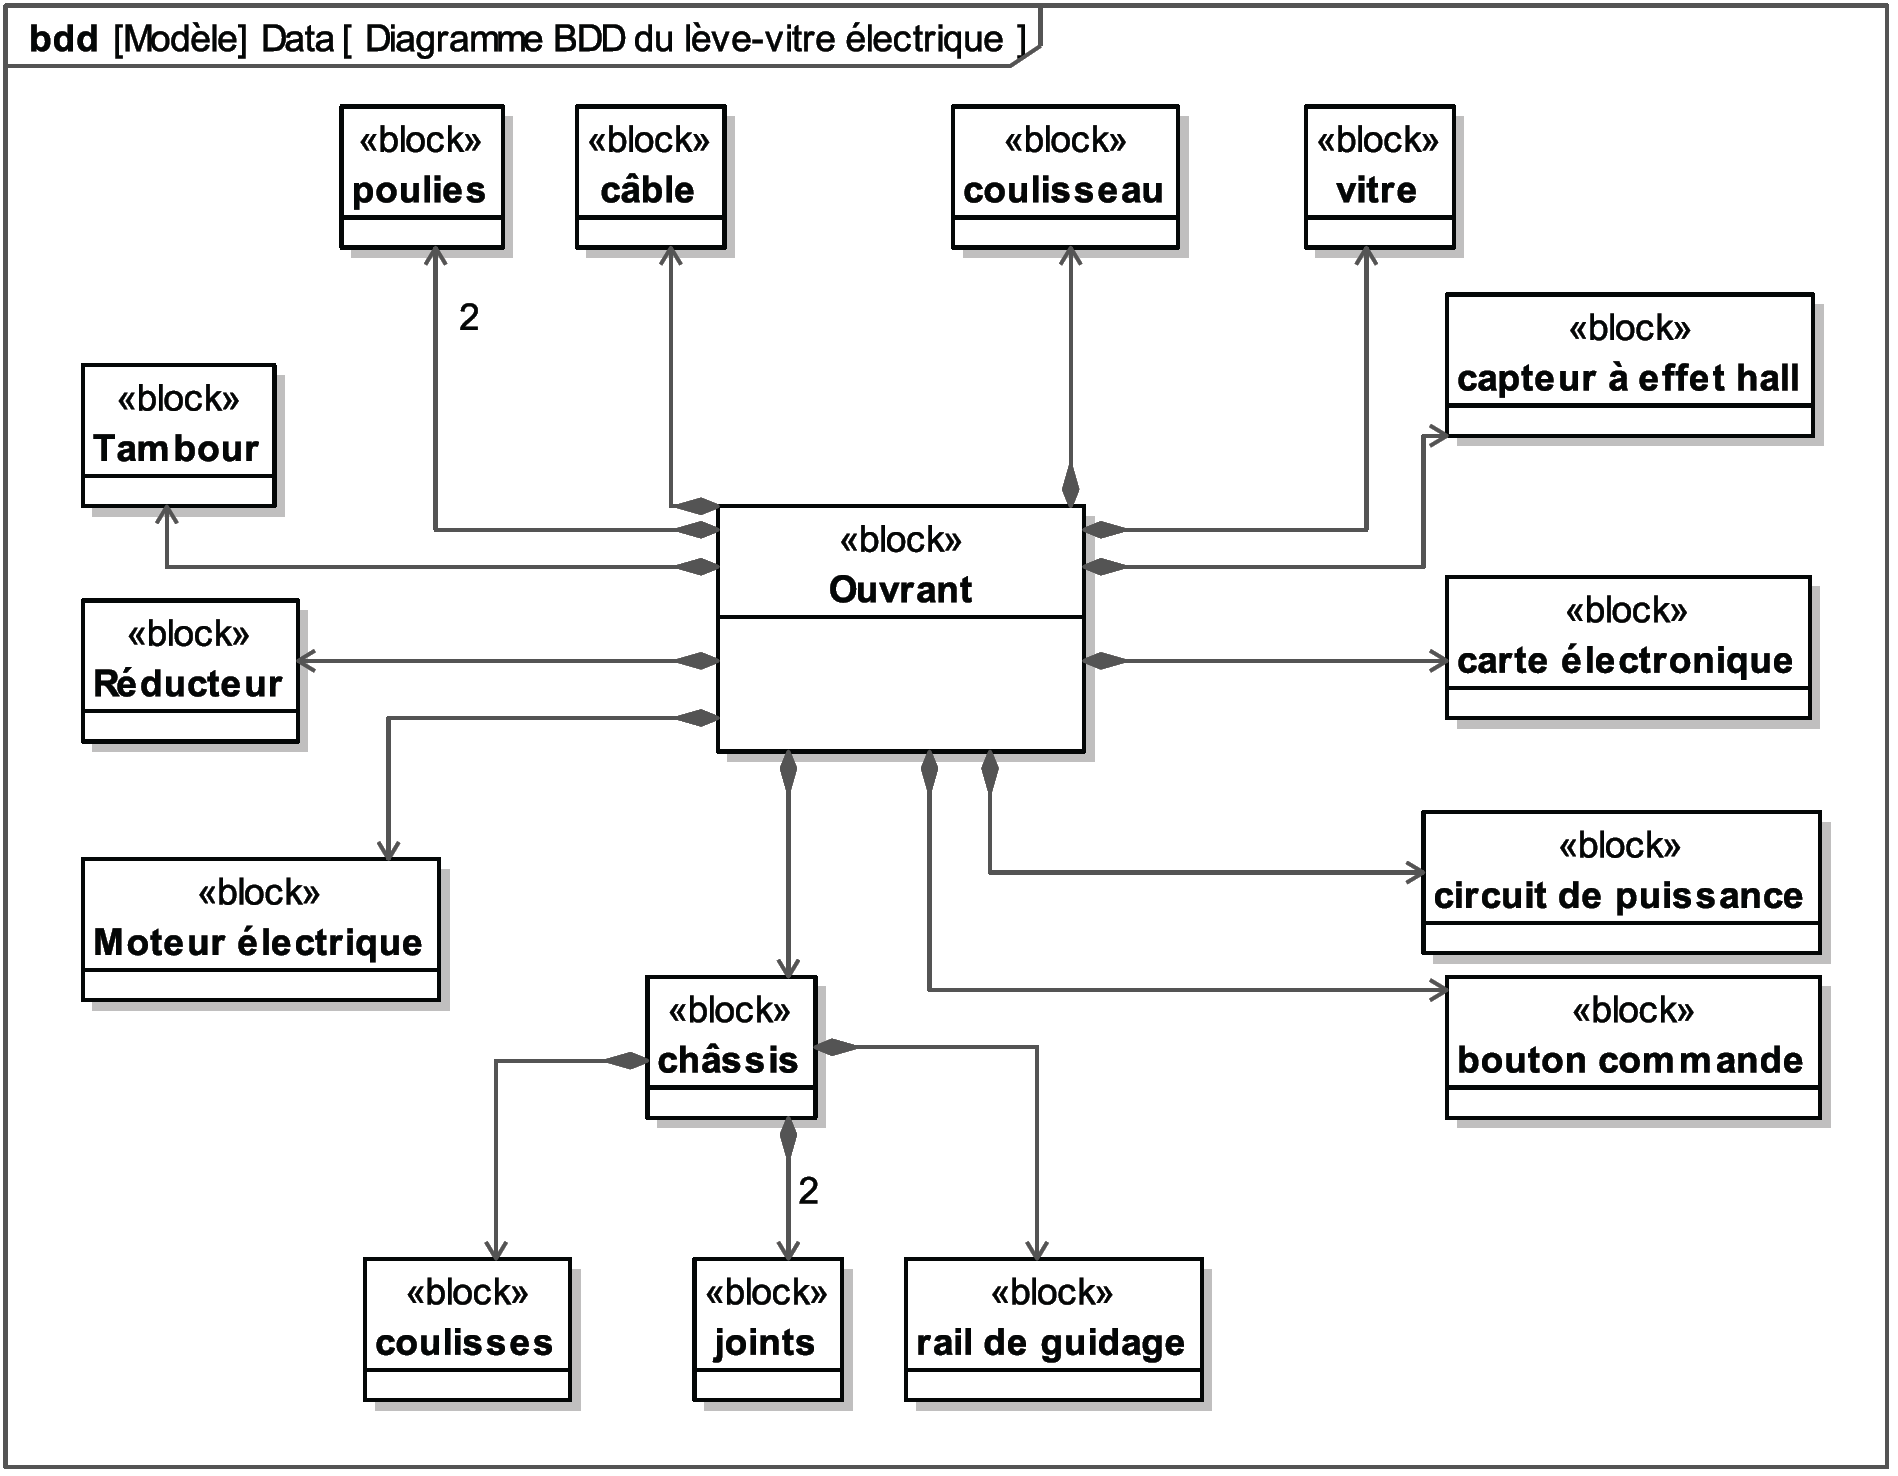
\includegraphics[width=0.8\linewidth]{img/img04}
 \caption{Diagramme de définitions de blocs (BDD) du lève-vitre électrique}
 \label{img04}
\end{figure}

On note $v(t)$ la vitesse de déplacement en translation de la vitre et $\omega_m(t)$ la vitesse angulaire du moteur, avec: $v(t)=\frac{D}{2}.\frac{1}{Z}.\omega_m(t)$.

\paragraph{Question 2:}	Déterminer l'expression littérale du rapport de réduction $r$ (roue et vis + poulie) tel que
$v(t) = r.\omega_m(t)$. Effectuer l'application numérique. On prendra dans la suite la valeur $r=0,39mm.rad^{-1}$.

\paragraph{Question 3:} Déterminer le nombre de tours $N_t$ que doit faire le moteur pour obtenir le déplacement de la vitre indiqué dans le diagramme des exigences.

\paragraph{Question 4:} Sachant que le régime nominal du moteur est de $4000tr.min^{-1}$, en déduire la durée (en $s$) d'ouverture/fermeture $\Delta_o$ de la fenêtre. Conclure quant à l'exigence correspondante du diagramme des exigences.

%\subsection{Modélisation du guidage: Guidage d'une porte coulissante}
%
%\begin{figure}[!h]
%\begin{minipage}{0.45\linewidth}
%La structure de la porte coulissante électrique est proche de celle du lève-vitre (figure \ref{img08}). Un moto-réducteur entraîne, par l'intermédiaire d'un tambour et de poulies/câble, la porte qui est guidée par trois rails (inférieur, milieu et supérieur) grâce à trois chariots en liaison avec la porte. Des galets (trois par chariot) sont montés sur ces chariots pour assurer le guidage avec les rails. La chaîne d'information de la porte coulissante est exactement la même que pour le lève- vitre. Le diagramme BDD de la porte coulissante est donné sur la figure \ref{img09}.
%\end{minipage}
%\begin{minipage}{0.45\linewidth}
% \centering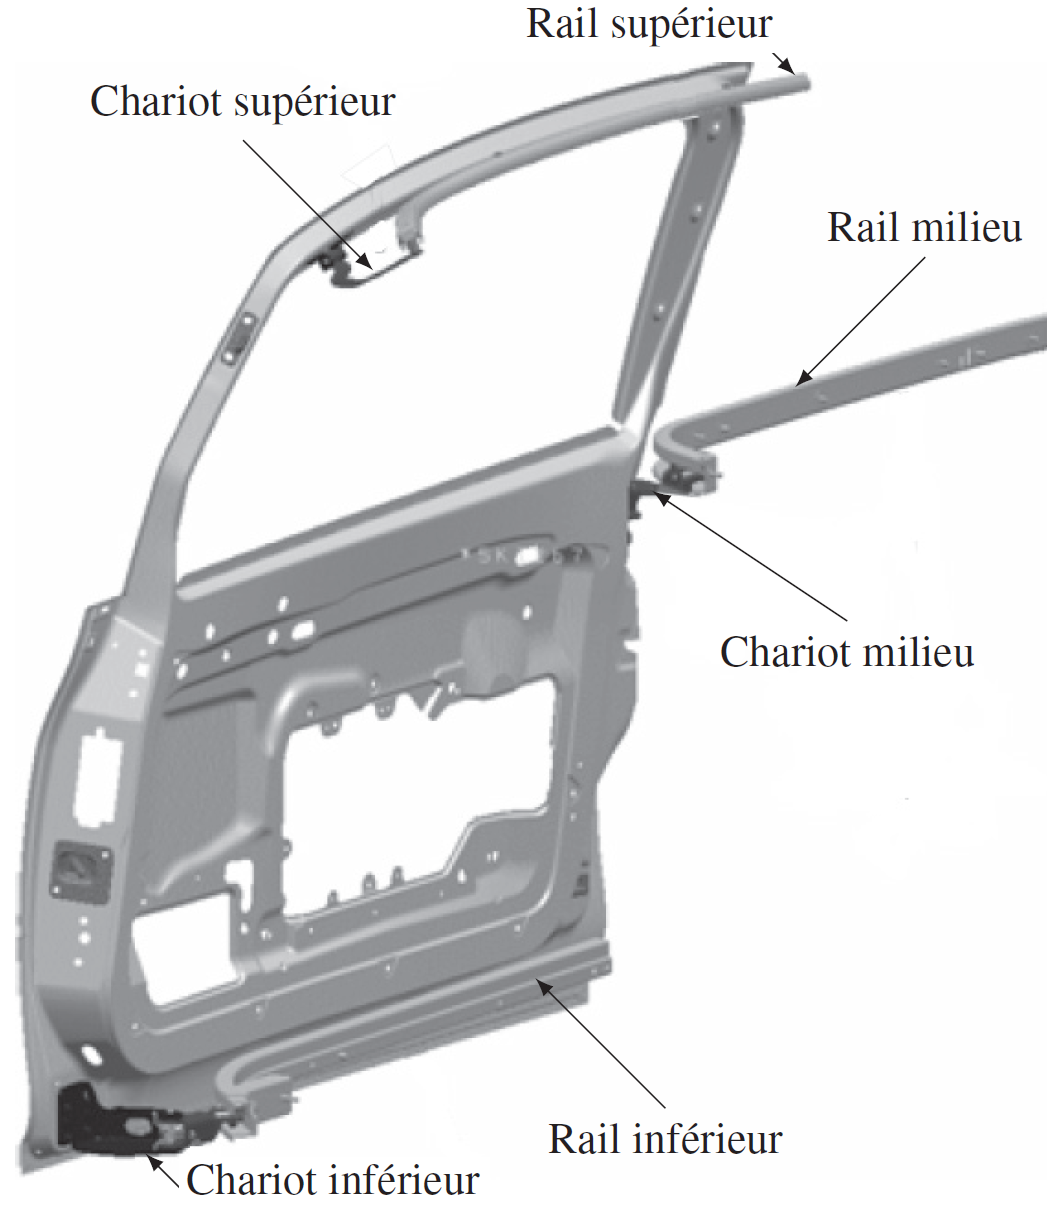
\includegraphics[width=0.8\linewidth]{img/img08}
% \caption{Description du système de guidage de la porte coulissante électrique}
% \label{img08}
%\end{minipage}
%\end{figure}
%
%\begin{figure}[!h]
% \centering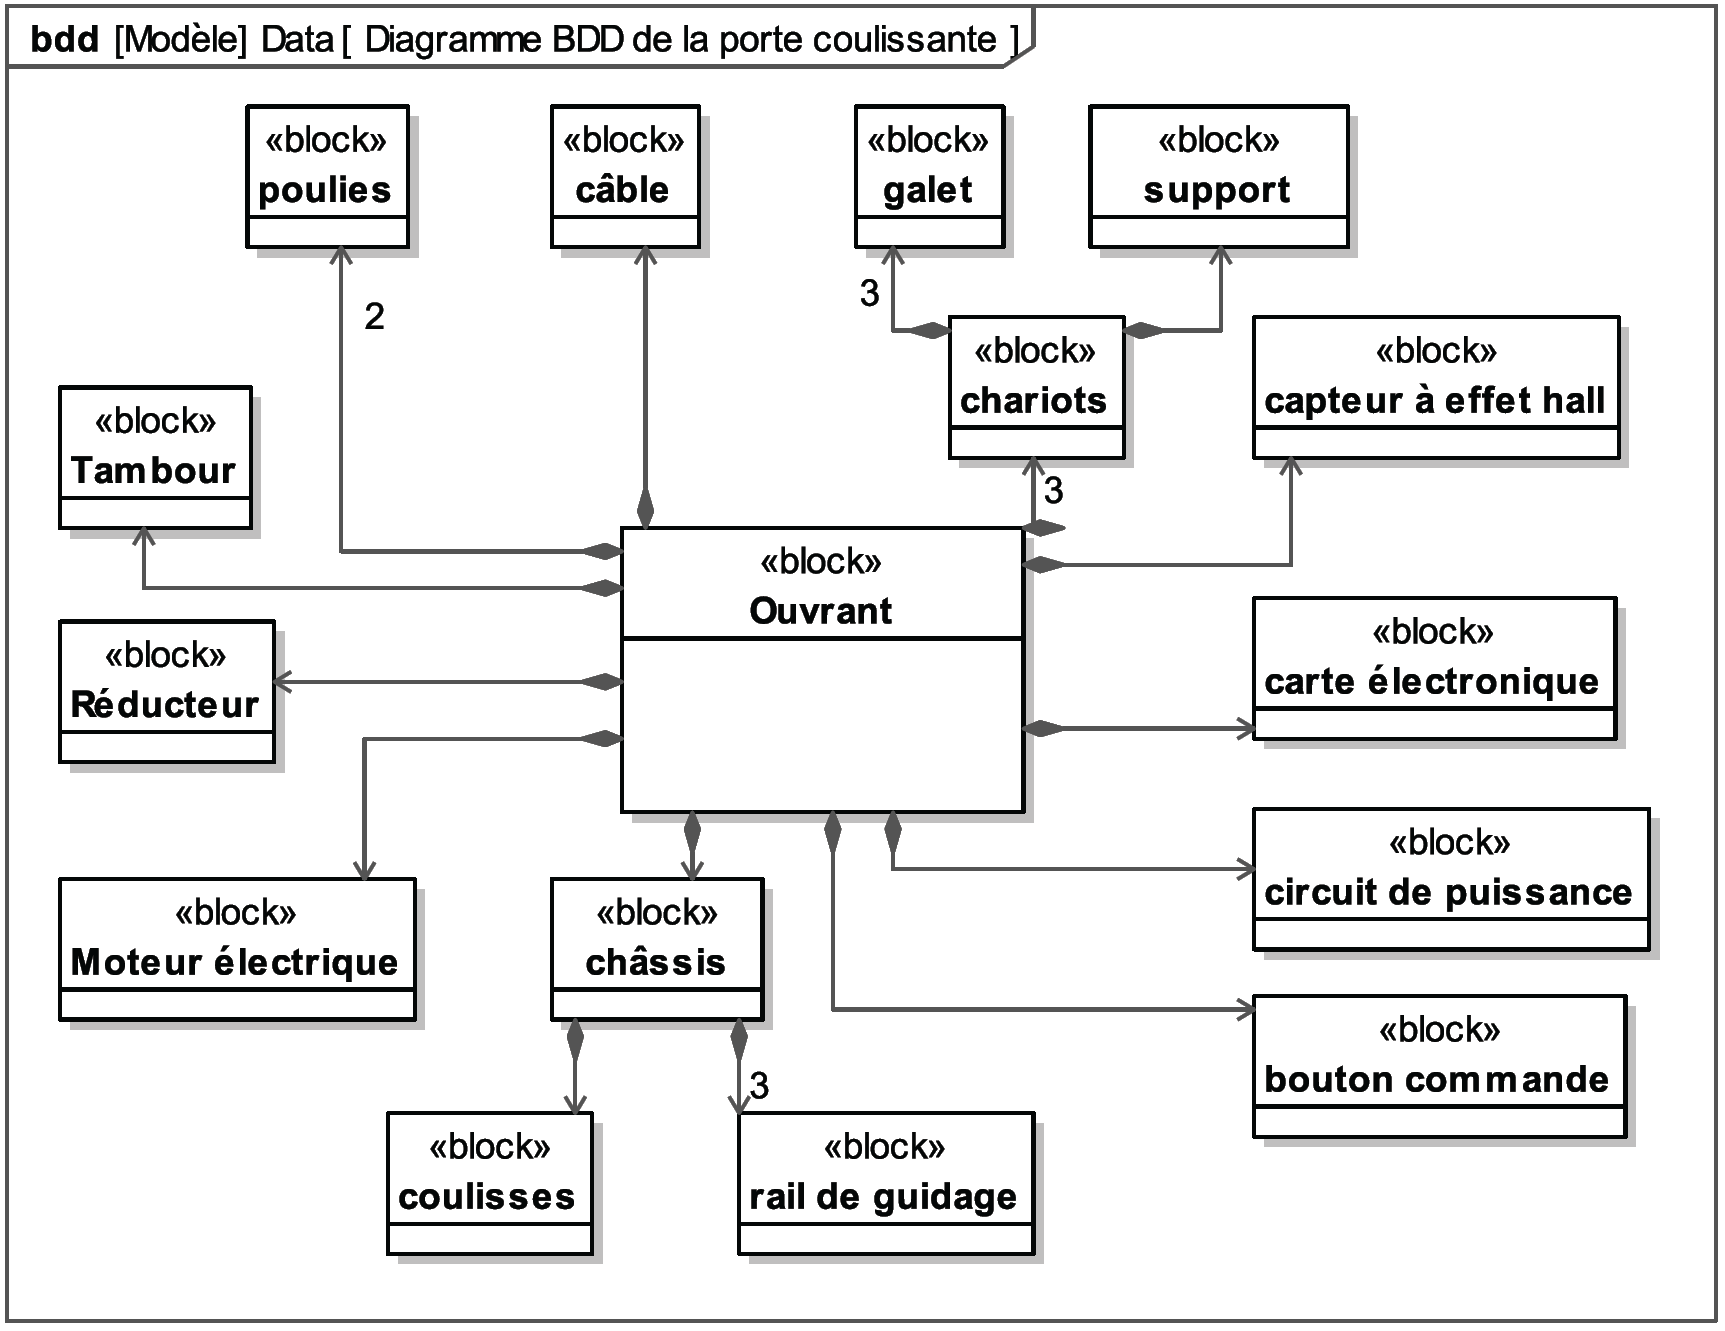
\includegraphics[width=0.8\linewidth]{img/img09}
% \caption{Diagramme BDD de la porte coulissante}
% \label{img09}
%\end{figure}

\section{Commande asservie}

La partie précédente a permis de mettre en évidence une méthode de détection de pincement dans le cadre d'une commande tout ou rien en boucle ouverte. La plupart des ouvrants sont commandés de cette manière. Cependant, de nouvelles fonctionnalités ou contraintes définies dans le cahier des charges peuvent nécessiter la prise en compte d'une commande asservie de vitesse. C'est le cas, par exemple, de la porte coulissante où la vitesse est variable et contrôlée selon les moments de fonctionnement.

La méthode précédente doit être modifiée car l'asservissement doit réagir pour maintenir une vitesse fixée, ce qui est contraire à la détection d'un obstacle. La nouvelle méthode consiste à développer un estimateur de l'effort dû à l'obstacle et à utiliser cette information pour détecter l'obstacle.

\subsection{Mise en place de l'asservissement de vitesse}

On considère la vitre de masse $m$ se déplaçant verticalement. Le moment d'inertie du rotor autour de son axe de rotation est noté $J_m$. Les inerties, autres que celles de la vitre et du rotor, sont négligées. On appelle $\omega_m(t)$ la vitesse angulaire du rotor du moteur et $r$ le rapport de réduction entre la vitesse $v(t)$ de la vitre et la vitesse angulaire du moteur : $v(t) = r.\omega_m(t)$.

Le référentiel lié à la voiture est supposé galiléen. On pose :
\begin{itemize}
 \item $f_v$ le coefficient de frottement visqueux de l'axe du moteur,
 \item $C_r(t)$ le couple résistant ramené au niveau de l'axe du moteur. Celui-ci prend en compte les frottements (autre que ceux dans le moteur), la pesanteur et aussi la présence ou non d'un obstacle, ce sont les seules pertes. Toutes les autres liaisons seront considérées comme parfaites,
 \item $C_m(t)$ le couple exercé par le moteur.
\end{itemize} 

En appliquant le théorème de l'énergie cinétique à l'ensemble en mouvement on peut montrer que:

\begin{center}
$J.\frac{d\omega_m(t)}{dt}+f_v.\omega_m(t)=C_m(t)-C_r(t)$ (1)
\end{center}
avec $J=J_m+m.r^2$

Les équations qui caractérisent le moteur à courant continu sont : $u_m(t)=R.i(t)+k_e.\omega_m(t)$ (2) et $C_m(t)=k_c.i(t)$ (3) avec $R$, $k_e$ et $k_c$ des constantes caractéristiques du moteur.

\paragraph{Question 5:} Passer les équations (1), (2) et (3) dans le domaine de Laplace.

\paragraph{Question 6:} En déduire les fonctions de transfert $H_1(p)$ et $H_2(p)$ telles que $\Omega_m(p)=H_1(p).U_m(p)+H_2(p).C_r(p)$

\paragraph{Question 7:} Mettre ces fonctions de transfert sous leurs formes canonique et en déduire les caractéristiques $K_1$, $\tau_1$, $K_2$ et $\tau_2$.

\paragraph{Question 8:} Déterminer leurs ordres et leurs classes.

~\

La valeurs numériques des caractéristiques du système sont indiquées sur le document réponse.

\paragraph{Question 9:} Comme cela a été fait pour la première ligne $R$, indiquer l'unité de la variable considérée. 

\paragraph{Question 10:} Compléter le tableau du document réponse en indiquant les unités de chacune des variables à partir de unités de base du système international. 

\paragraph{Question 11:} Déterminer les valeurs numériques des composantes $K_1$, $\tau_1$, $K_2$ et $\tau_2$.
 
~\

On donne:
\begin{itemize}
 \item $S_1(p)=H_1(p).U_m(p)$
 \item $S_2(p)=H_2(p).C_r(p)$
\end{itemize}

\paragraph{Question 12:} En utilisant la décomposition en éléments simples déterminer $s_1(t)$ la réponse temporelle à un échelon $u_m(t)=12V$.

\paragraph{Question 13:} Par identification, en utilisant les résultats de la question précédente, déterminer $s_2(t)$ la réponse temporelle à un échelon $C_r(t)=0,2N.m$.

\paragraph{Question 14:} En déduire $\omega_m(t)=s_1(t)+s_2(t)$ la réponse du système. Tracer cette réponse sur le document réponse et mettre sur ce tracé toutes les constructions nécessaires à son interprétation.

~\

La figure \ref{img15}, présente le schéma-blocs de l'asservissement avec :
\begin{itemize}
 \item deux entrées $\Omega_c(p)$ vitesse angulaire de consigne du moteur et $C_r(p)$ couple résistant,
 \item une sortie $\Omega_m(p)$.
\end{itemize}


\begin{figure}[!h]
 \centering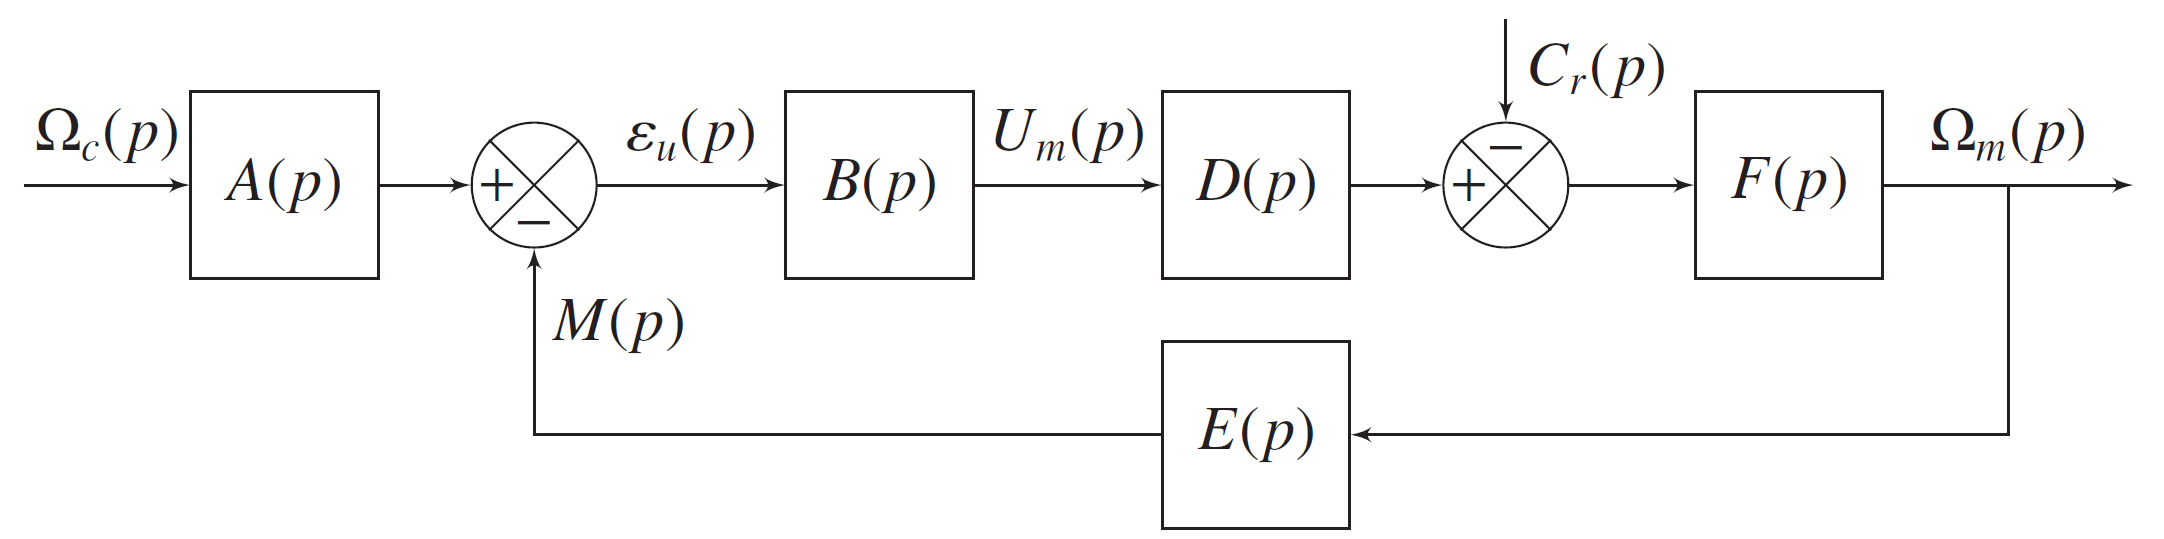
\includegraphics[width=0.9\linewidth]{img/img15}
 \caption{Schéma-blocs de l'asservissement de vitesse du moteur}
 \label{img15}
\end{figure}

\paragraph{Question 15:} Déterminer les fonctions de transfert $D(p)$ et $F(p)$, en fonction de $H_1(p)$ et $H_2(p)$.

~\

On donne les données suivantes:
\begin{itemize}
 \item $B(p)=10$ (sans unité),
 \item $E(p)=0,01V.rad^{-1}.s$.
\end{itemize}

\paragraph{Question 16:} Déterminer la fonction de transfert du bloc $A(p)$ et faire l'application numérique.

~\

\newpage

Pour la suite, on prendra $C_r(p)=0$.

\paragraph{Question 17:} Déterminer $FTBO(p)=\frac{M(p)}{C(p)}$ et $FTBP(p)=\frac{\Omega(p)}{\Omega_c(p)}$. Mettre ces fonctions sous la forme canonique.

\paragraph{Question 18:} Donner l'ordre et la classe pour chacune d'elle. Identifier les valeurs caractéristiques de ces fonctions de transfert et faire l'application numérique.

\section{Système de commande d'un essuie-glace}

Le dessin donné dans le document réponse présente une solution de commande d'essuie-glace.

\paragraph{Question 19:} Colorier les classes d'équivalence sur le dessin d'ensemble et sur la nomenclature associée.

\begin{center}
FIN DU SUJET
\end{center}

\newpage

\section{Annexes}

\begin{figure}[!h]
 \centering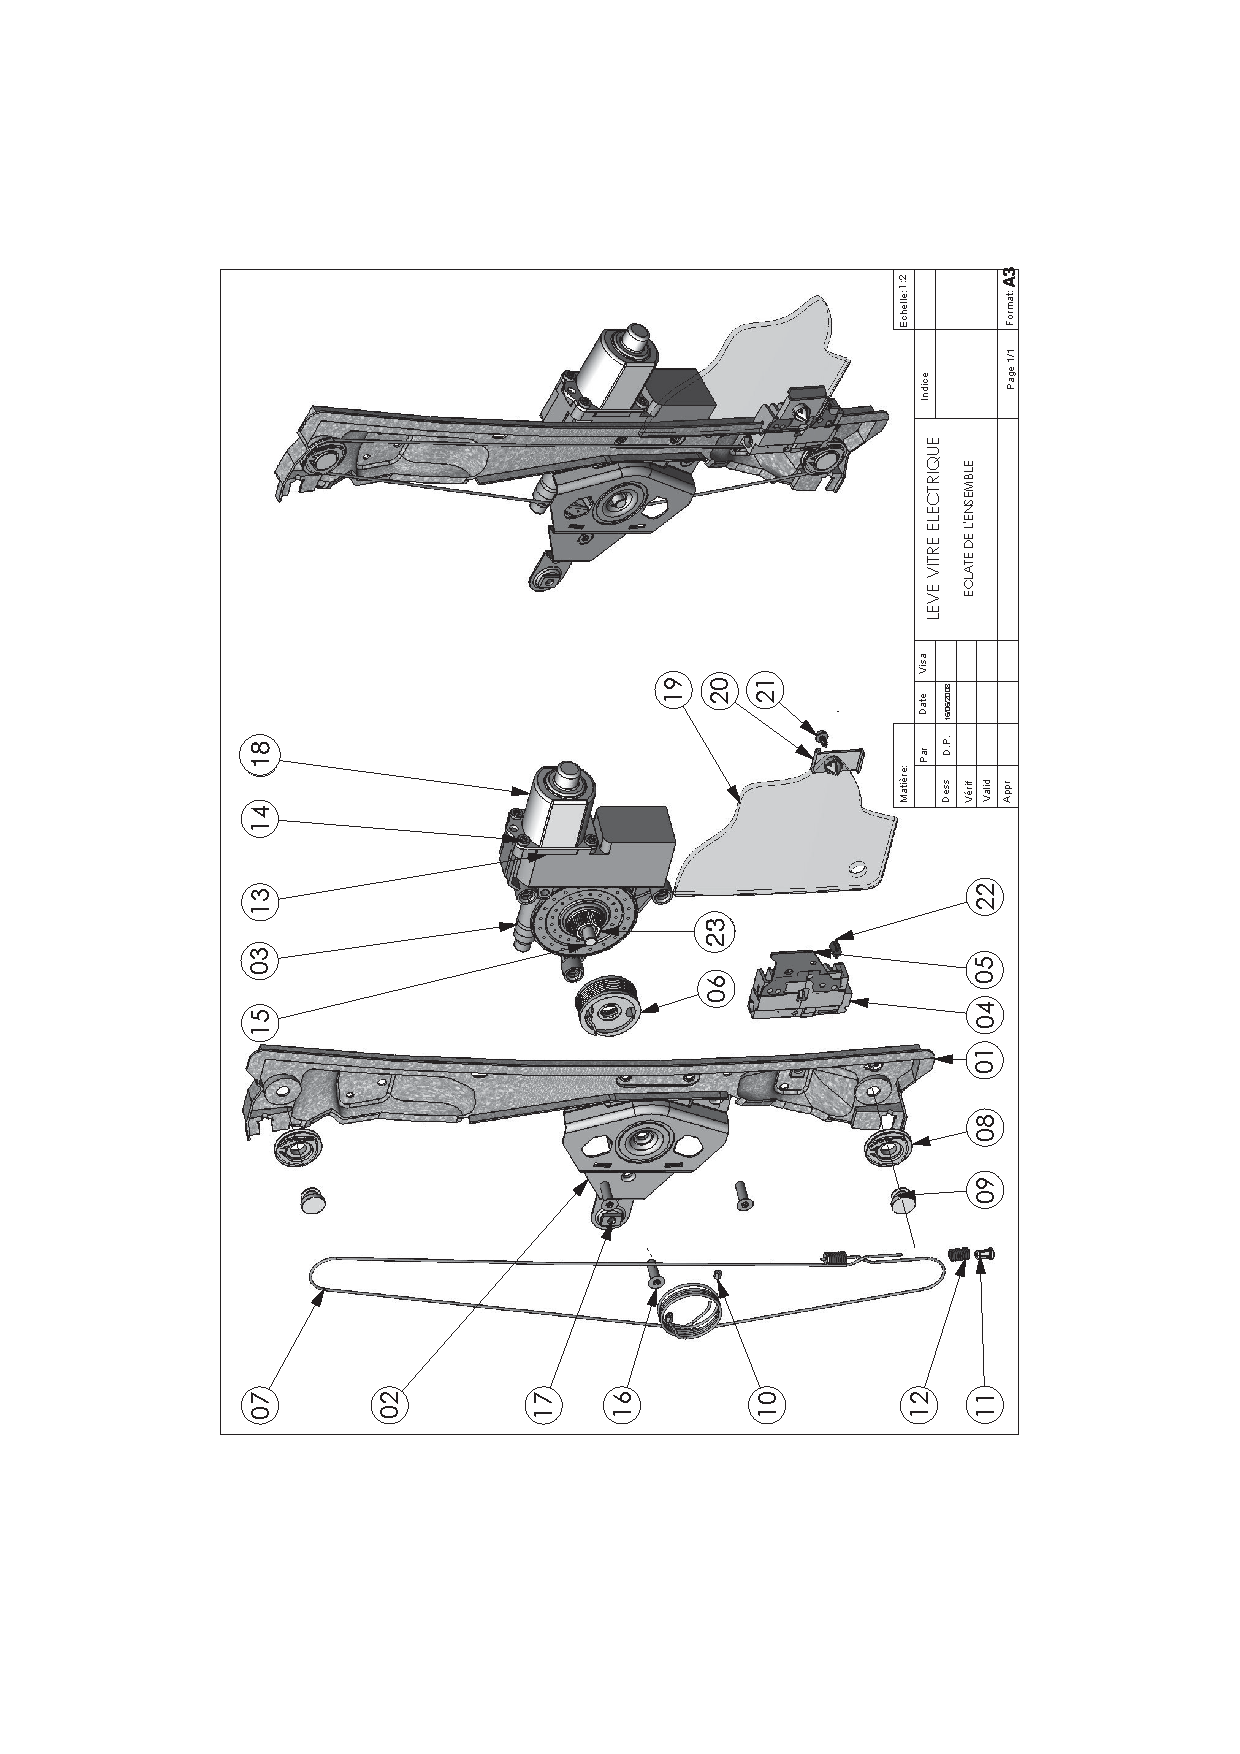
\includegraphics[width=0.9\linewidth]{img/eclate1}
 \caption{Éclaté de la structure interne du lève-vitre électrique}
 \label{an01}
\end{figure}

\begin{figure}[!h]
 \centering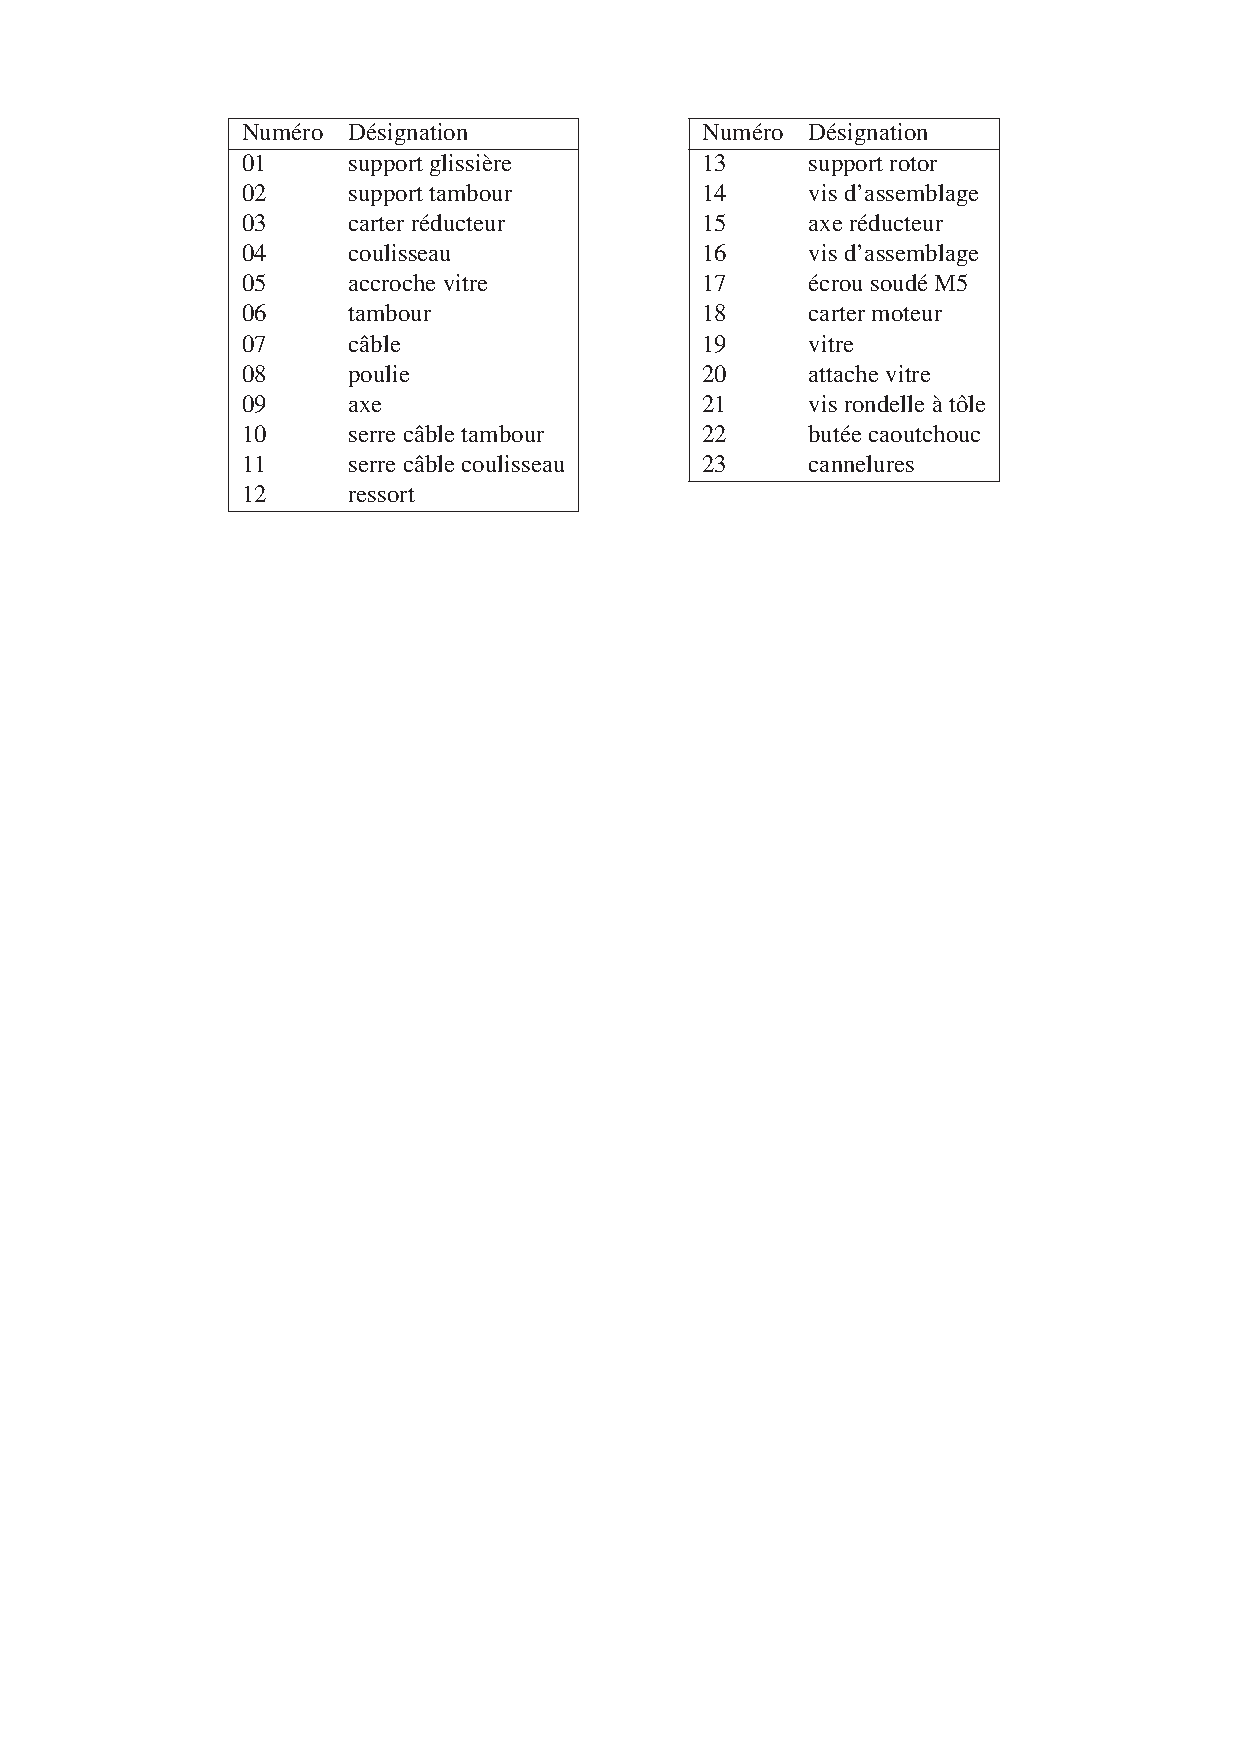
\includegraphics[width=0.9\linewidth]{img/eclate1_2}
 \caption{Nomenclature}
 \label{an011}
\end{figure}

\begin{figure}[!h]
 \centering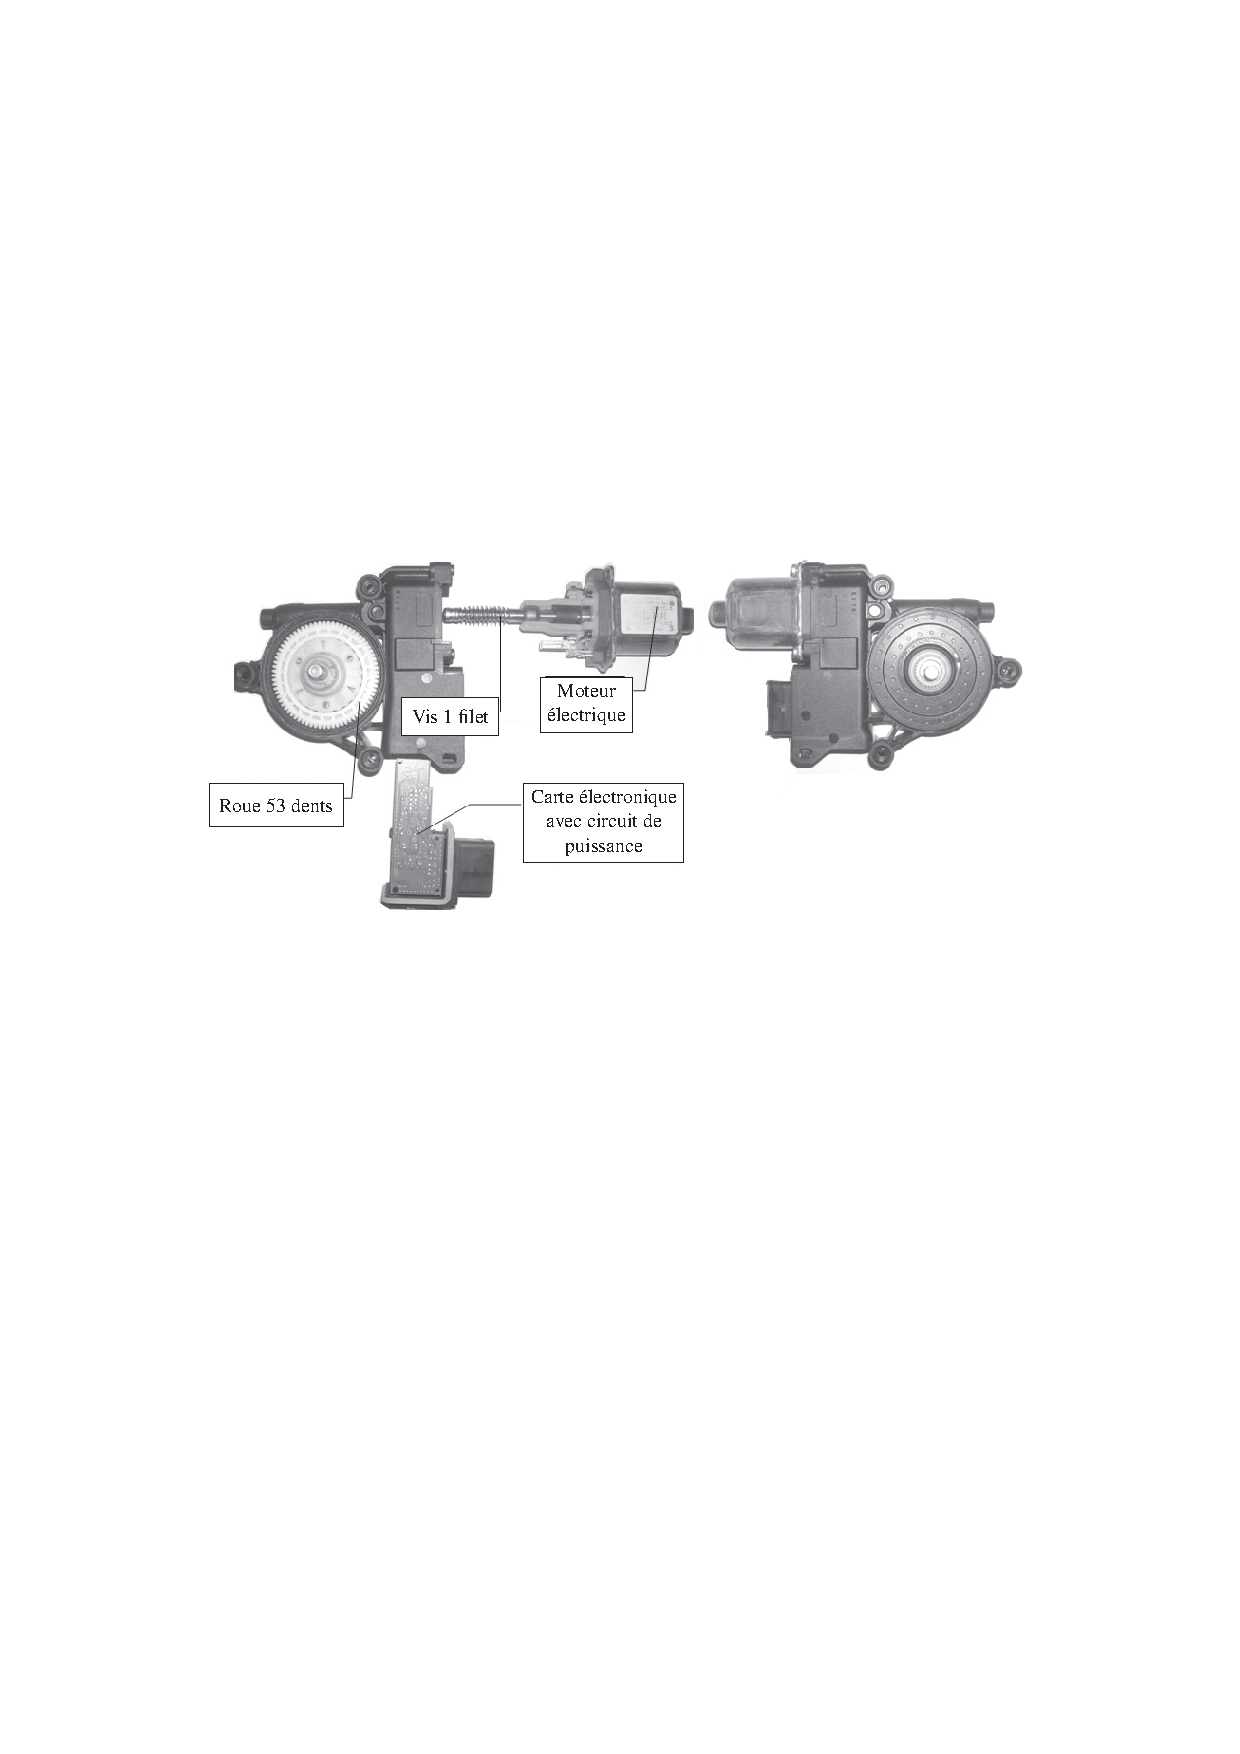
\includegraphics[width=0.9\linewidth]{img/eclate2}
 \caption{ du moto-réducteur}
 \label{an02}
\end{figure}


\newpage
\cleardoublepage

\pagestyle{documentreponse}

\section{Documents réponse}

\reponse{1}{0}

\begin{center}
 \centering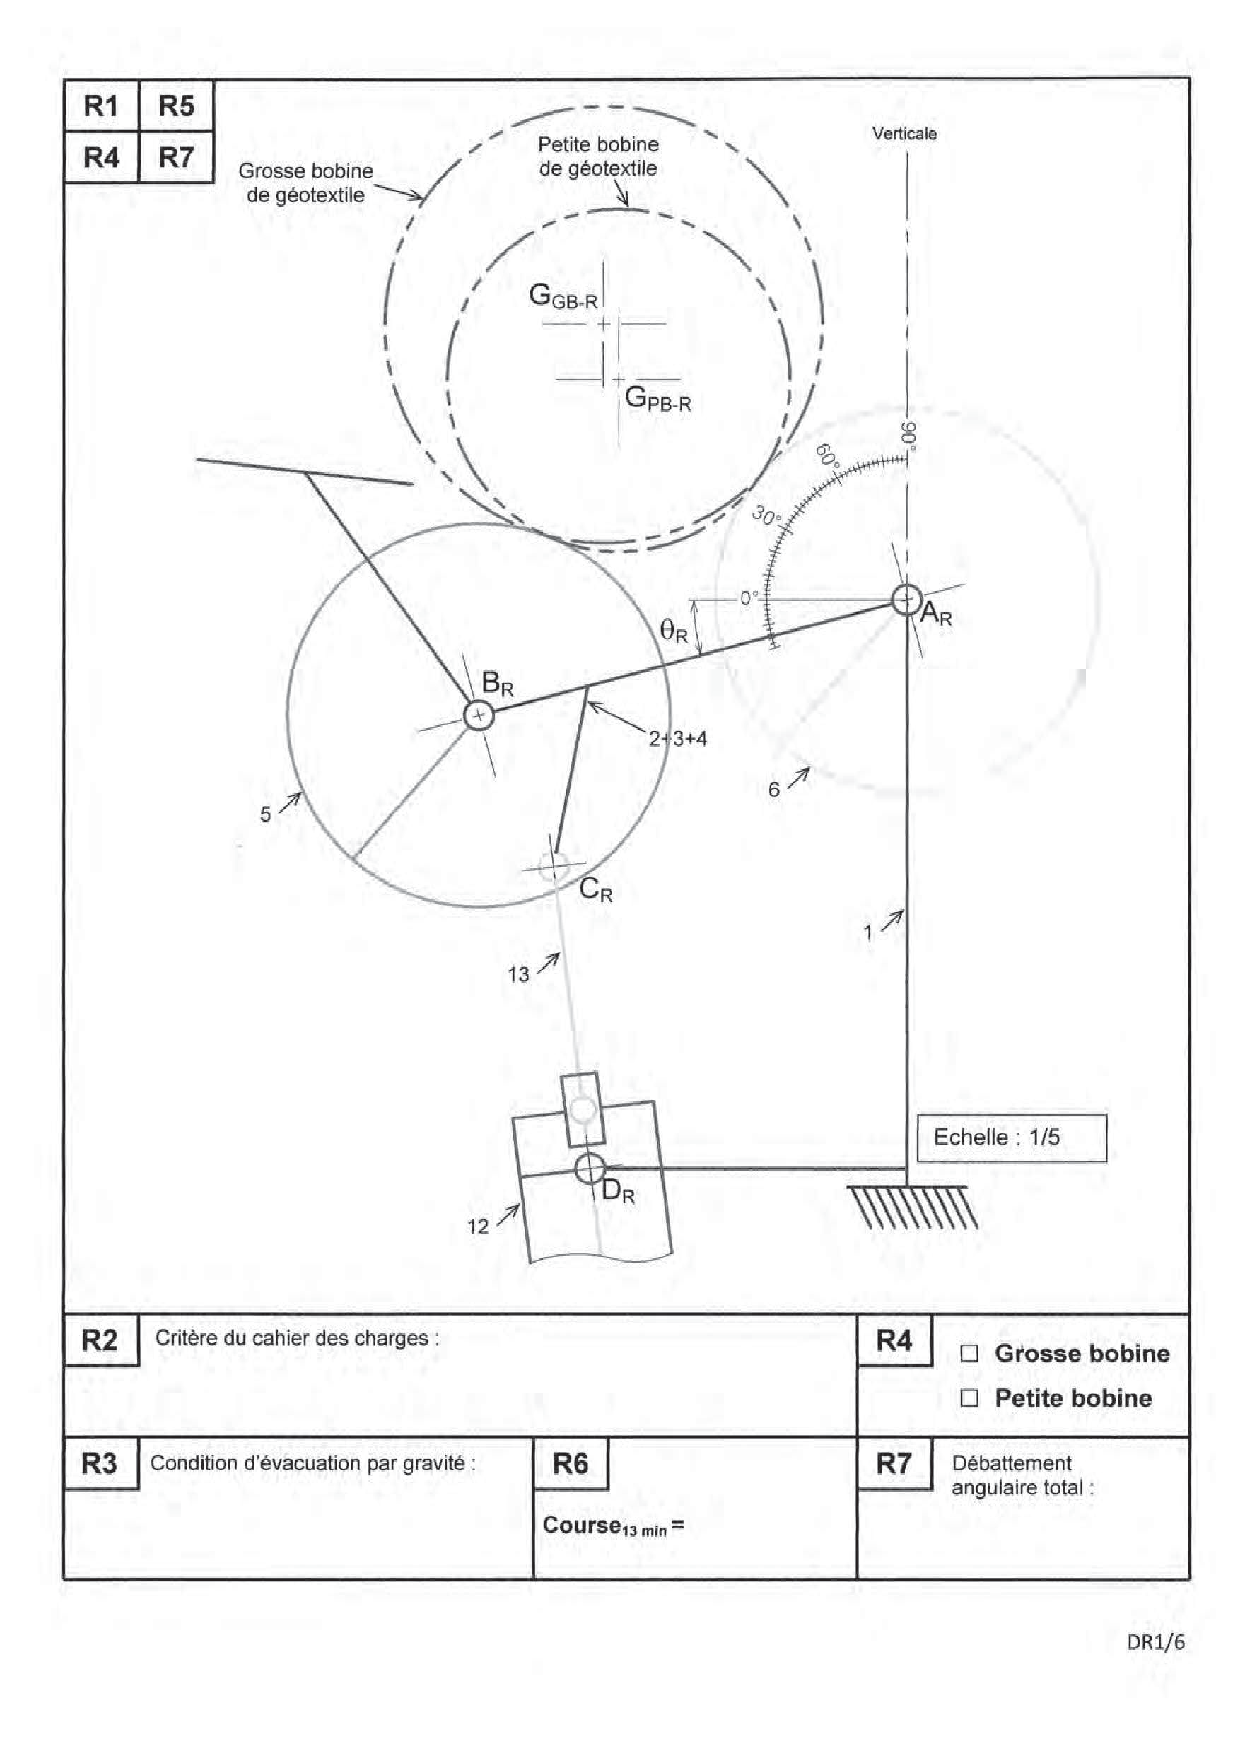
\includegraphics[width=0.99\linewidth]{img/dr1}
\end{center}

\reponse{2}{7}

\reponse{3}{6}

\reponse{4}{7}

\reponse{5}{9}

\reponse{6}{12}

\reponse{7}{6}

\reponse{8}{4}

\reponse{9}{0}

\begin{center}
\begin{tabular}{|c|c||c|c|c|c|}
\hline
$R$ & $2$ & $V$ & & $\Omega$ & X \\
\hline
$k_e$ & $52,5.10^{-3}$ & $V.s$ & & $N.m.A^{-1}$ & \\
\hline
$k_c$ & $52,5.10^{-3}$ & $V.s$ & & $N.m.A^{-1}$ & \\
\hline
$J_m$ & $0,01$ & $kg.m^2$ & & $kg.m^2.s^{-2}$ & \\
\hline
$m$ & 5 & $kg$ & & $N$ & \\
\hline
$f_v$ & 0,125 & $N.m$ & & $N.m.s$ & \\
\hline
\end{tabular}
\end{center}

\reponse{10}{0}

\begin{center}
\begin{tabular}{|c|m{3cm}|}
\hline
$R$ &  \\
\hline
$k_e$ &  \\
\hline
$k_c$ &  \\
\hline
$J_m$ &  \\
\hline
$m$ &  \\
\hline
$f_v$ & \\
\hline
\end{tabular}
\end{center}

\reponse{11}{4}

\reponse{12}{12}

\reponse{13}{6}

\reponse{14}{11}

\begin{center}
 \centering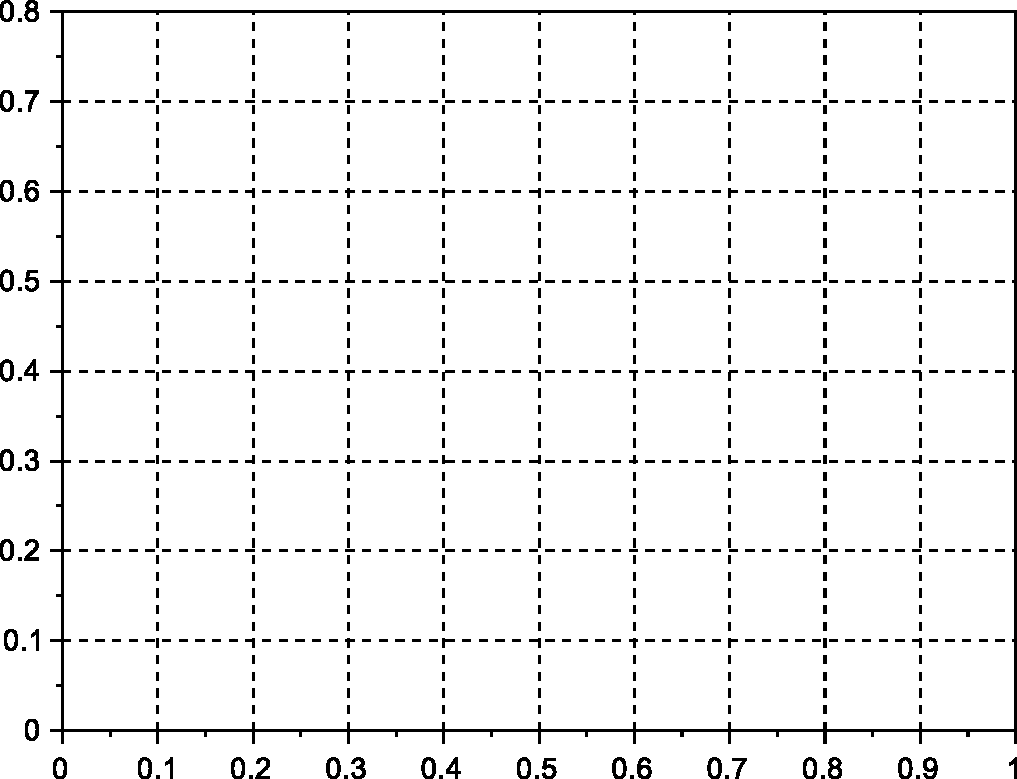
\includegraphics[width=0.8\linewidth]{img/temp_vide}
\end{center}

\reponse{15}{14}

\reponse{16}{6}

\reponse{17}{12}

\reponse{18}{11}


\reponse{19}{0}

\begin{center}
	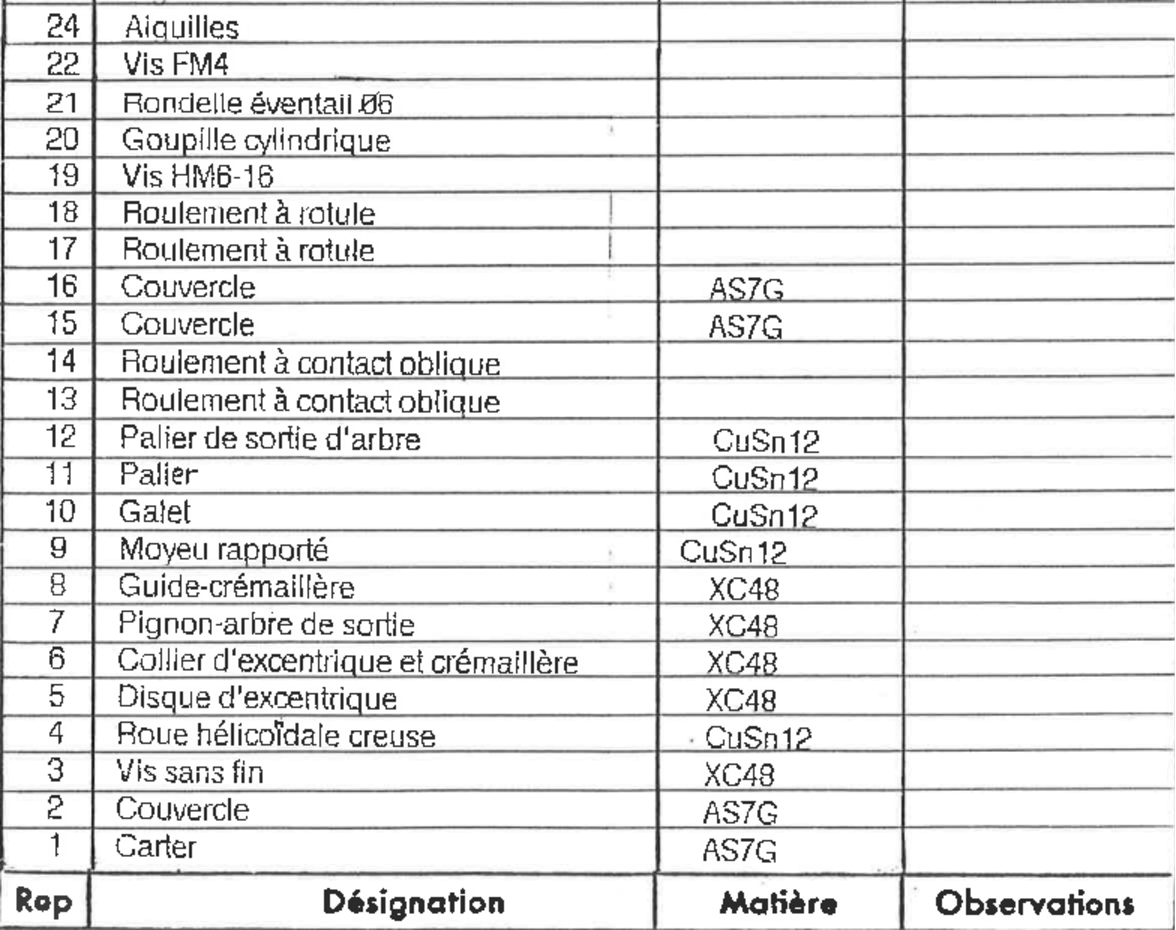
\includegraphics[width=0.7\linewidth]{img/Commande_essui_glace_nom.pdf}
\end{center}

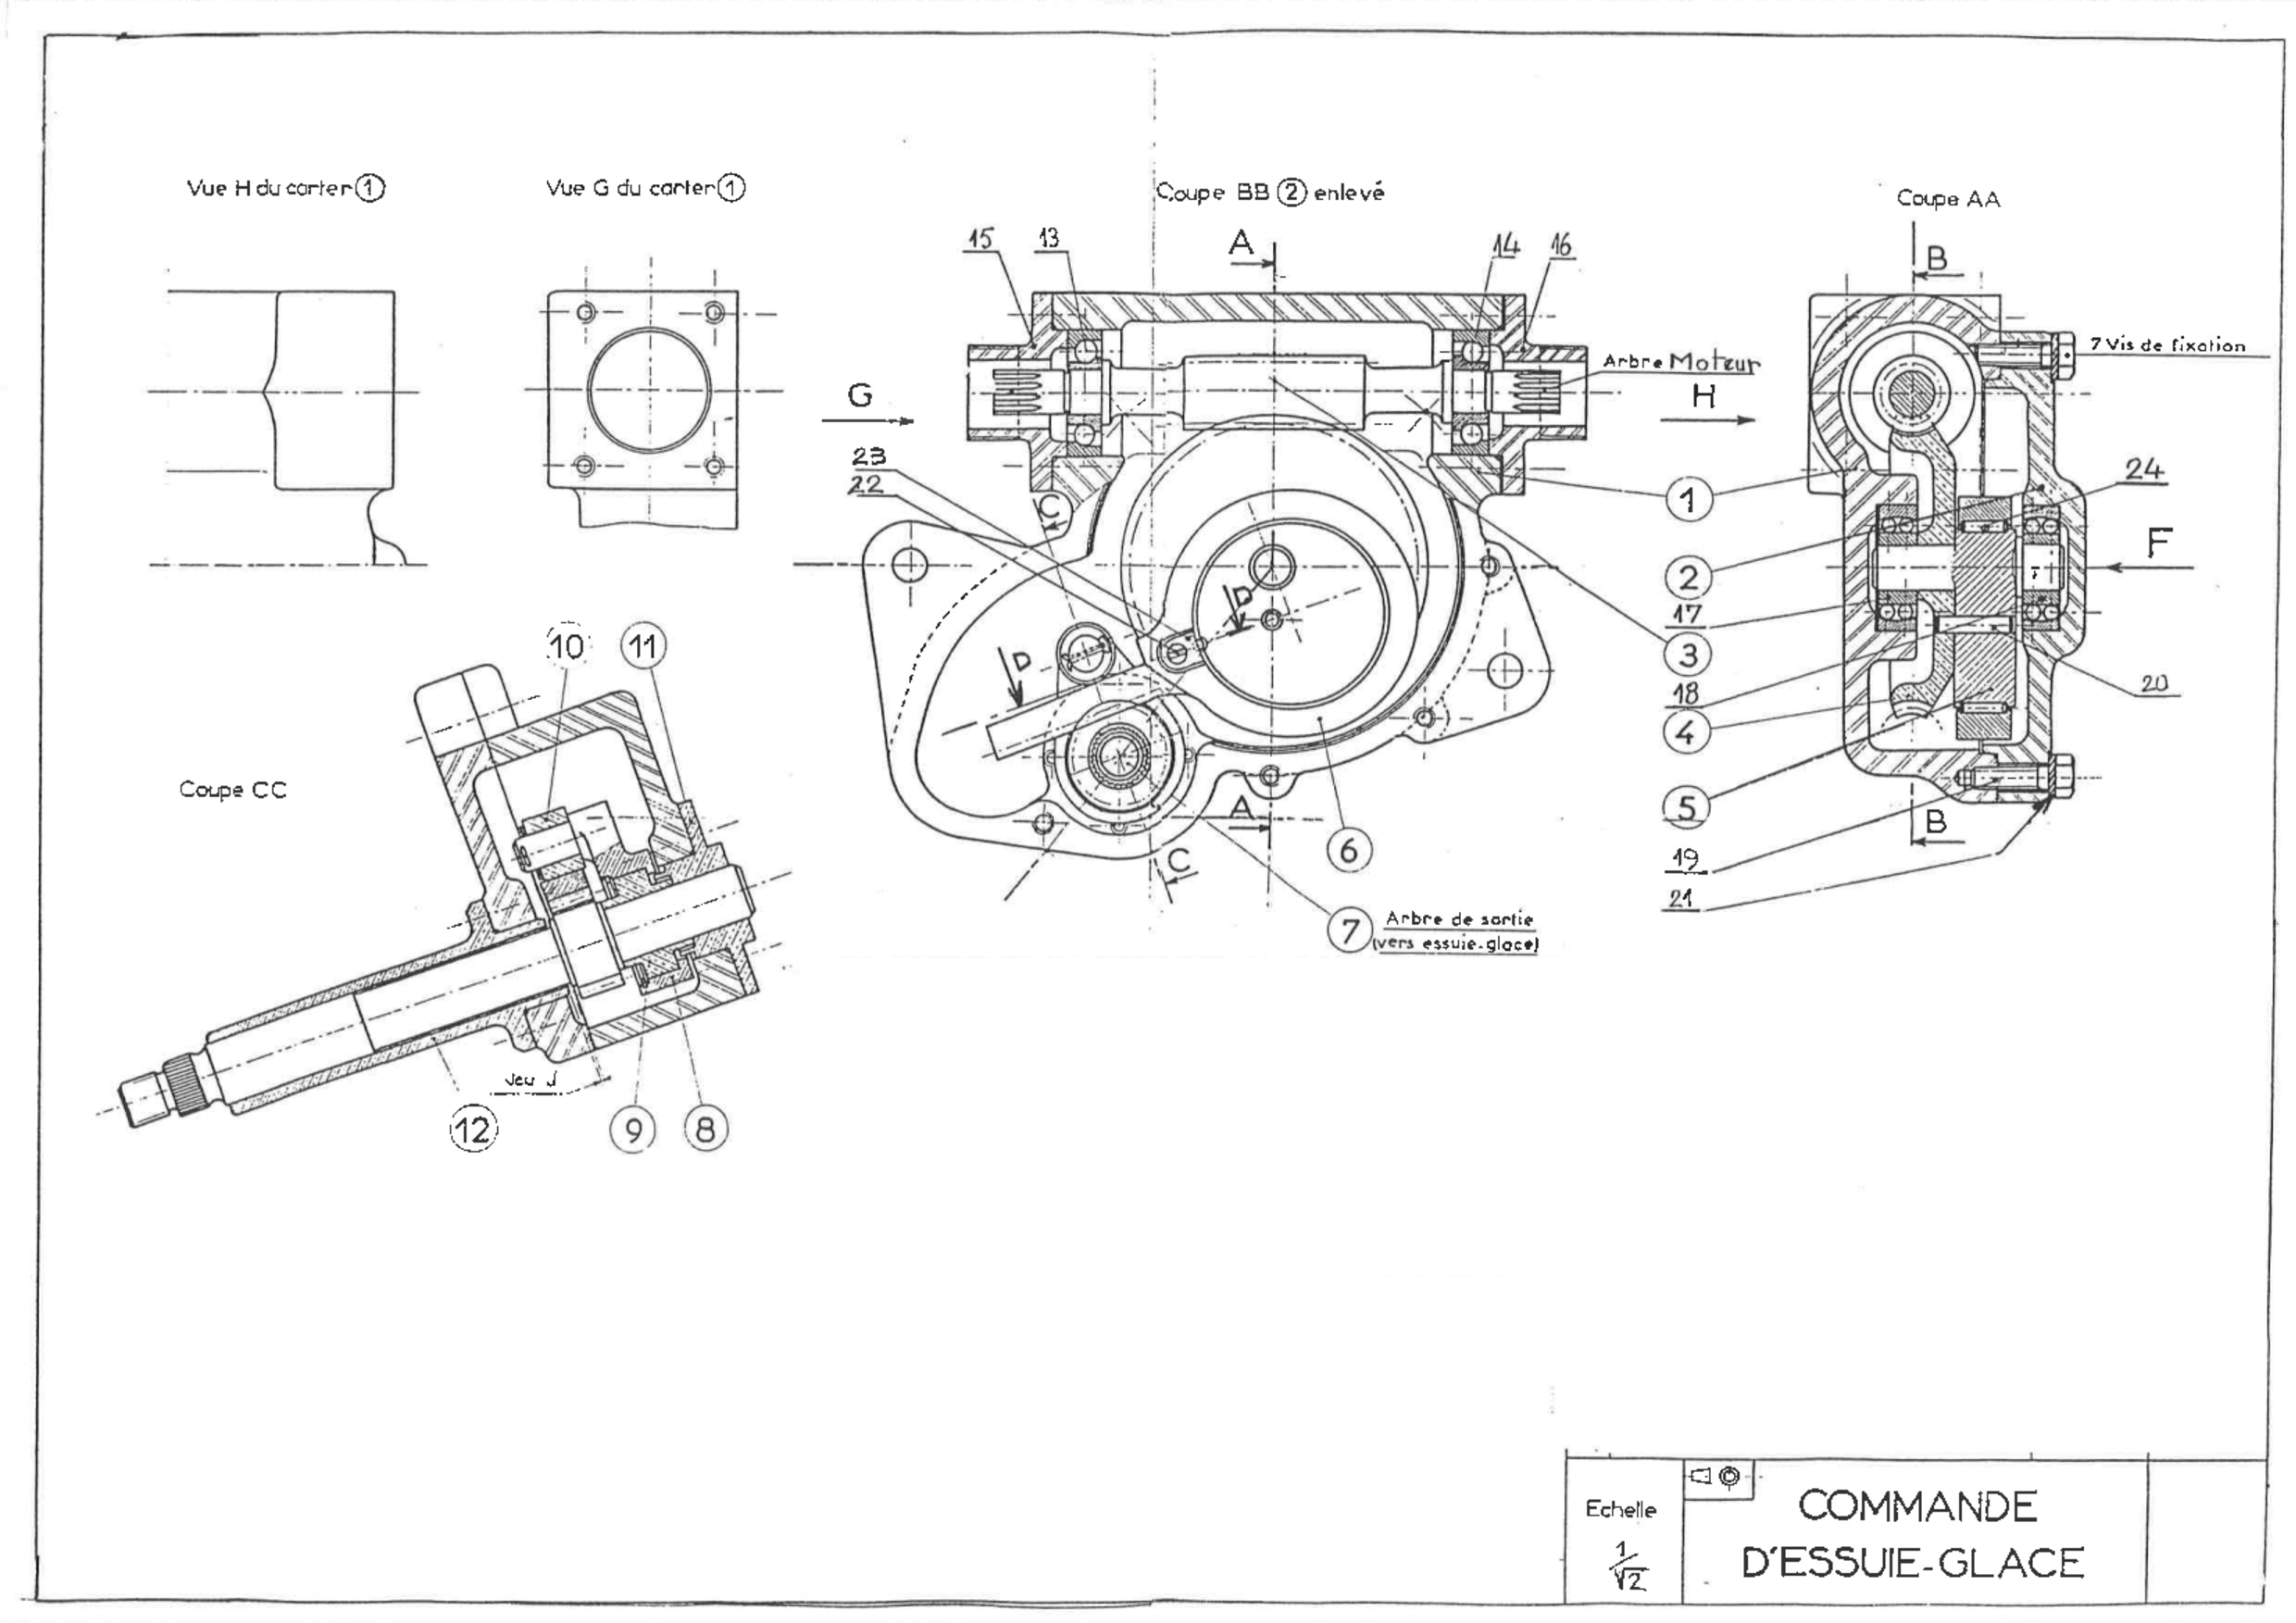
\includepdf[angle=90,offset=-6mm -8mm]{img/Commande_essui_glace_dessin.pdf}

\ifdef{\public}{\end{document}}{}

\newpage
\cleardoublepage

\pagestyle{correction}

\section{Correction}

\reponse{1}{0}

\begin{center}
 \centering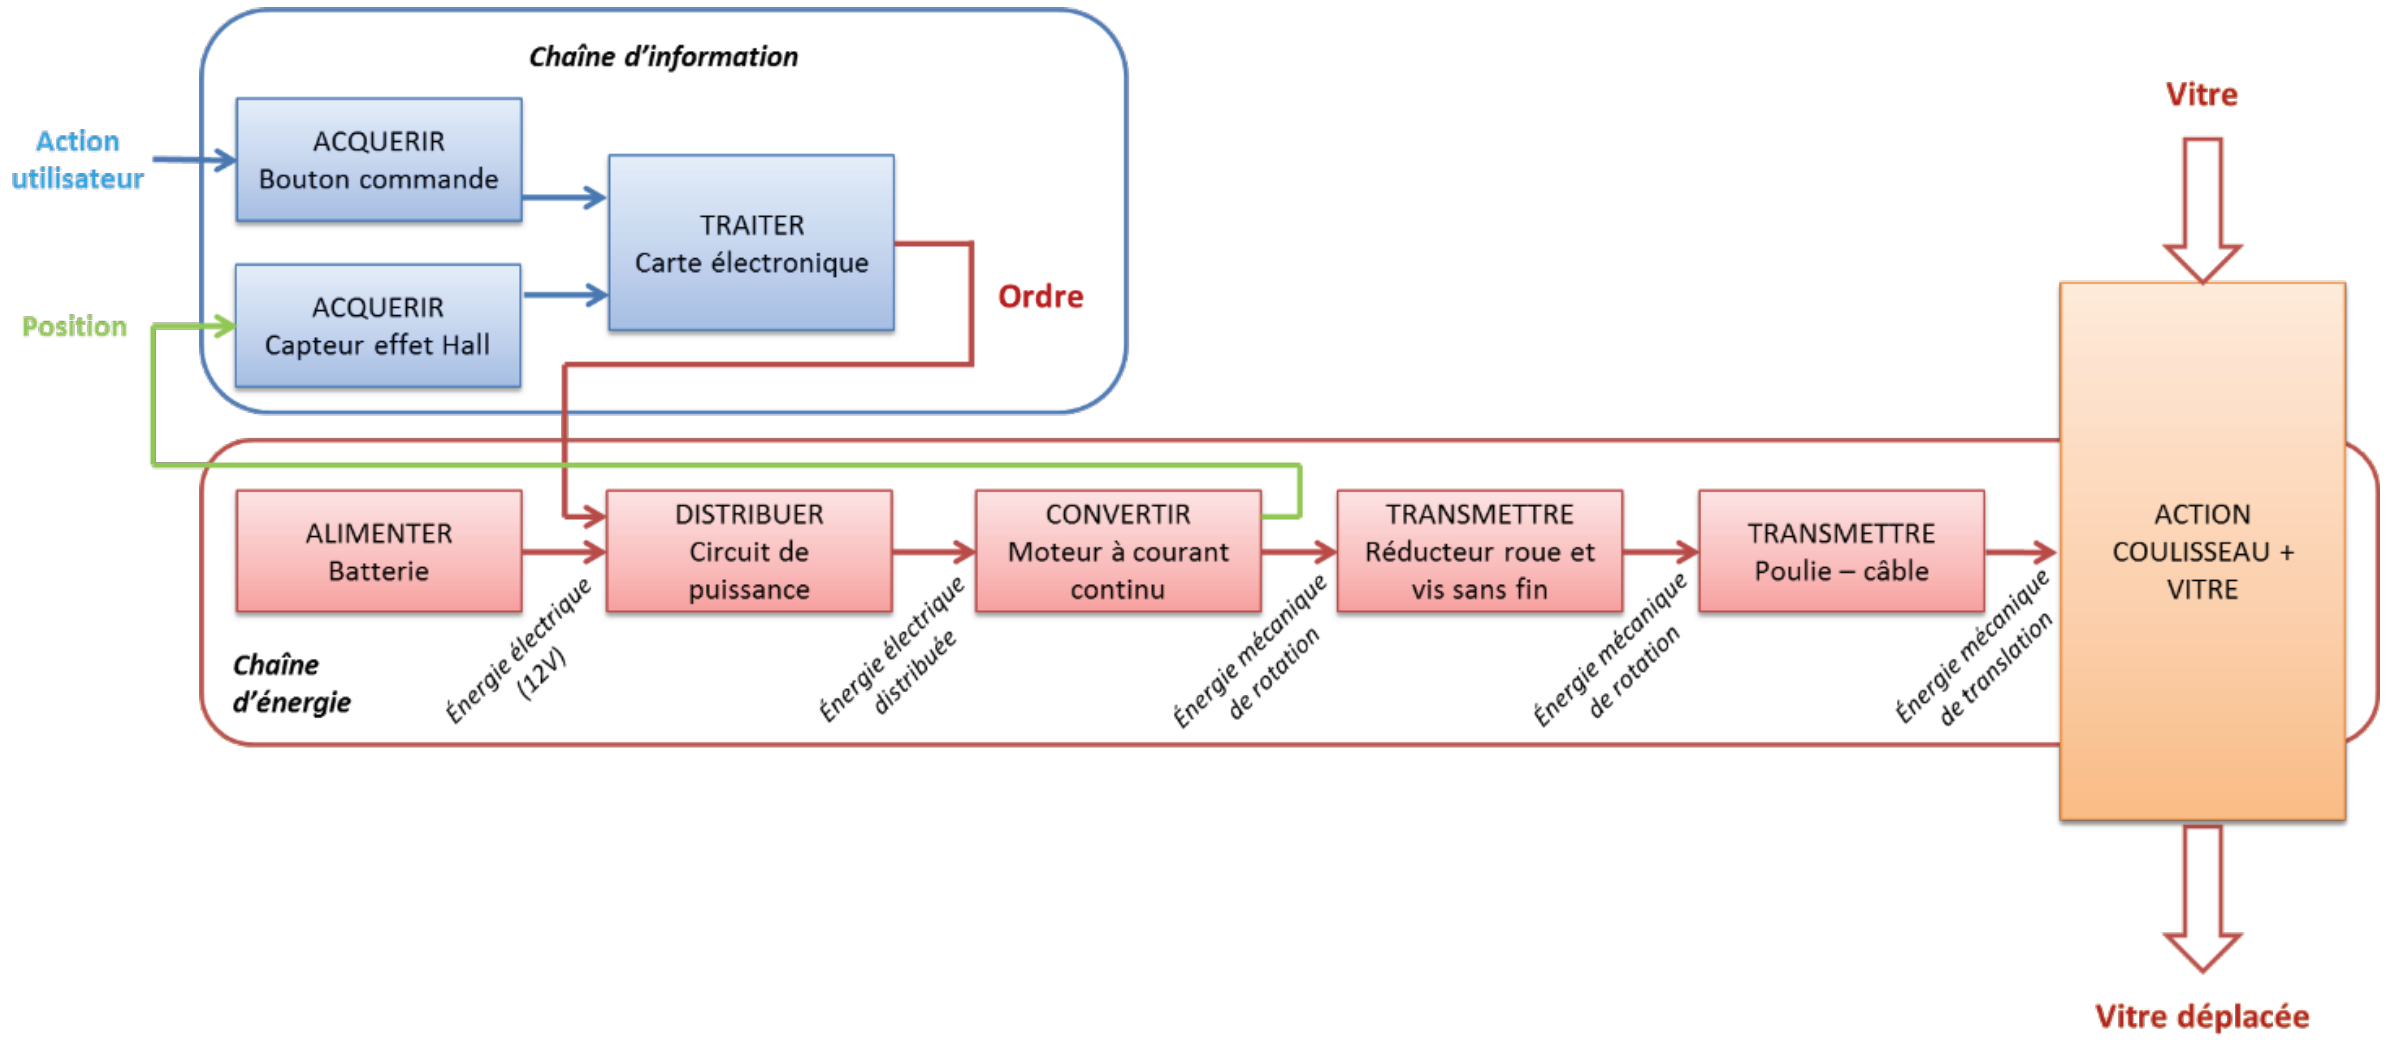
\includegraphics[width=0.9\linewidth]{img/dr1_cor}
\end{center}

\reponse{2}{0}

$r=\frac{D}{2.Z}=0,39mm.rad^{-1}$

\reponse{3}{0}

La distance à parcourir est de 45 cm (req 4.2). L'angle moteur est donc donné par $\theta_m=\frac{450}{r}=\frac{450}{0,4}\simeq 1125rad$, $N_t=183tours$

\reponse{4}{0}

À vitesse nominale on a $\Delta_o=\frac{\theta_m}{N_m}=\frac{183}{4000}=0,045min=2,7s$. Cette durée est inférieure aux 5 secondes fixées par l'exigence.

\reponse{5}{0}

$J.p.\Omega_m(p)+f_v.\Omega_m(p)=(J.p+f_v).\Omega_m(p)=C_m(p)-C_r(p)$ 

$U_m(p)=R.I(p)+k_e.\Omega_m(p)$ 

$C_m(p)=k_c.I(p)$
 
\reponse{6}{0}

$U_m(p)=R.\frac{(J.p.+f_v).\Omega_m(p)+C_r(p)}{k_c}+k_e.\Omega_m(p)$ 

$U_m(p)-\frac{R}{k_c}.C_r(p)=\frac{R.(J.p.+f_v)+k_e.k_c}{k_c}.\Omega_m(p)$ 

$\Omega_m(p)=\frac{k_c}{R.(J.p.+f_v)+k_e.k_c}.(U_m(p)-\frac{R}{k_c}.C_r(p))$ 

$\Omega_m(p)=\frac{k_c}{R.(J.p.+f_v)+k_e.k_c}.U_m(p)-\frac{R}{R.(J.p.+f_v)+k_e.k_c}.C_r(p)$ 

Donc, $H_1(p)=\frac{k_c}{R.(J.p.+f_v)+k_e.k_c}$ et $H_2(p)=-\frac{R}{R.(J.p.+f_v)+k_e.k_c}$.

\reponse{7}{0}

$H_1(p)=\dfrac{\frac{k_c}{R.f_v+k_e.k_c}}{1+\frac{R.J}{R.f_v+k_e.k_c}.p}$ et $H_2(p)=-\dfrac{\frac{R}{R.f_v+k_e.k_c}}{1+\frac{R.J}{R.f_v+k_e.k_c}.p}$.

$K_1=\frac{k_c}{R.f_v+k_e.k_c}$, $\tau_1=\frac{R.J}{R.f_v+k_e.k_c}$, $K_2=-\frac{R}{R.f_v+k_e.k_c}$ et $\tau_2=\frac{R.J}{R.f_v+k_e.k_c}$.

\reponse{8}{0}

Elles sont toutes les deux d'ordre 1 et de classe 0.

\reponse{9}{0}

\begin{center}
\begin{tabular}{|c|c||c|c|c|c|}
\hline
$R$ & $2$ & $V$ & & $\Omega$ & X \\
\hline
$k_e$ & $50.10^{-3}$ & $V.s$ & X & $N.m.A^{-1}$ & \\
\hline
$k_c$ & $50.10^{-3}$ & $V.s$ & & $N.m.A^{-1}$ & X \\
\hline
$J_m$ & $0,01$ & $kg.m^2$ & X & $kg.m^2.s^{-2}$ & \\
\hline
$m$ & 5 & $kg$ & X & $N$ & \\
\hline
$f_v$ & 0,125 & $N.m$ & & $N.m.s$ & X \\
\hline
\end{tabular}
\end{center}

\reponse{10}{0}

\begin{center}
\begin{tabular}{|c|c|}
\hline
$R$ & $A^{-2}.kg.m^2.s^{-3}$ \\
\hline
$k_e$ & $kg.m^2.s^{-2}.A^{-1}$ \\
\hline
$k_c$ & $kg.m^2.s^{-2}.A^{-1}$ \\
\hline
$J_m$ & $kg.m^2$ \\
\hline
$m$ & $kg$ \\
\hline
$f_v$ & $kg.m^2.s^{-1}$\\
\hline
\end{tabular}
\end{center}

\reponse{11}{0}

$K_1\simeq0.2V^{-1}.s^{-1}$, $\tau_1\simeq0,08s$, $K_2\simeq -8s^{-1}.N^{-1}.m^{-1}$ et $\tau_2\simeq0,08s$.

\reponse{12}{0}

$S_1(p)=H_1(p).E_1(p)=\frac{K_1}{1+\tau_1.p}.\frac{E_{1,0}}{p}=\frac{A}{1+\tau_1.p}+\frac{B}{p}=K_1.E_{1,0}.\left(\frac{1}{p}-\frac{\tau_1}{1+\tau_1.p}\right)$

$s_1(t)=K_1.E_{1,0}.(1-e^{-\frac{t}{\tau_1}})$.


\reponse{13}{0}

Par identification, $s_2(t)=K_2.E_{2,0}.(1-e^{-\frac{t}{\tau_2}})$

\reponse{14}{0}

$\omega_m(t)=s_1(t)+s_2(t)=K_1.E_{1,0}.(1-e^{-\frac{t}{\tau_1}})+K_2.E_{2,0}.(1-e^{-\frac{t}{\tau_2}})$.

On a $\tau_1=\tau_2$, donc $\omega(t)=(K_1.E_{1,0}+K_2.E_{2,0}).(1-e^{-\frac{t}{\tau_1}})$

$\omega(t)=(0,2.12-8.0,2).(1-e^{-\frac{t}{0,08}})=0,8.(1-e^{-\frac{t}{0,08}})$

\begin{center}
 \centering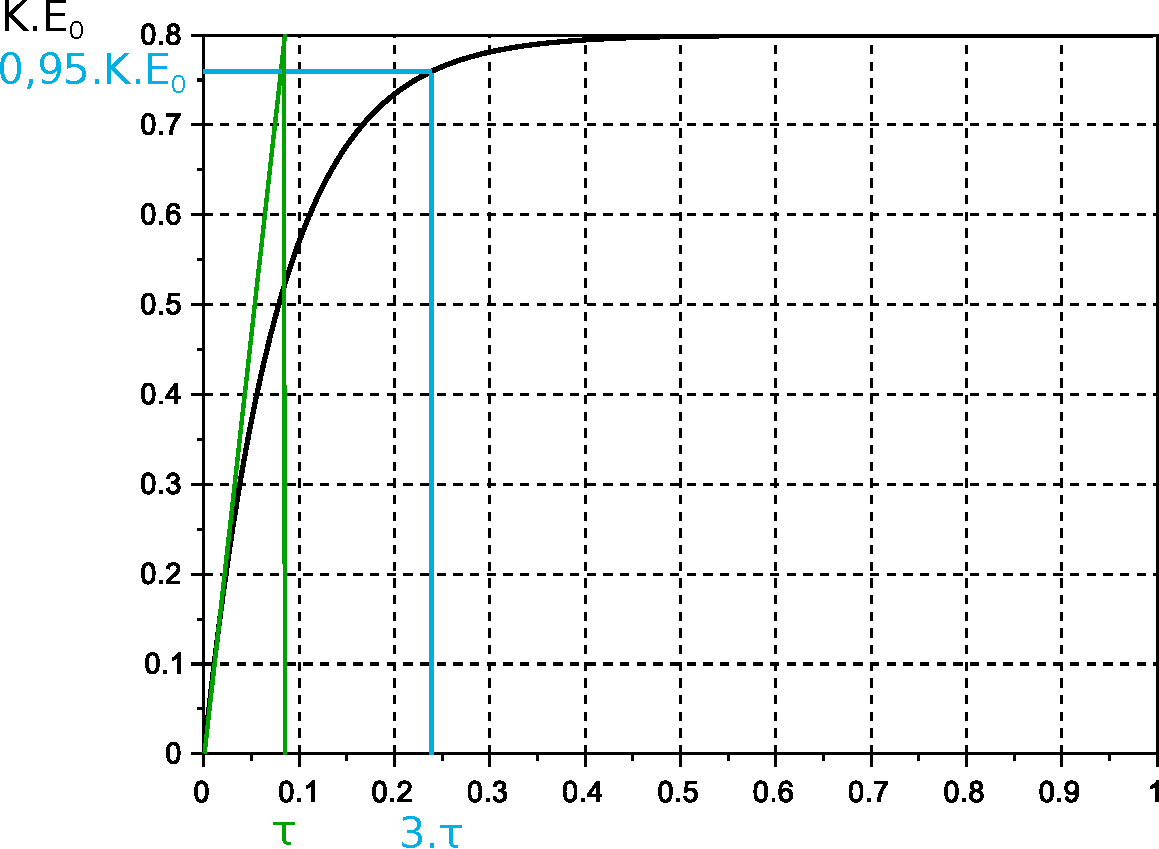
\includegraphics[width=0.9\linewidth]{img/temp_cor}
\end{center}

\reponse{15}{0}

$\left\{\begin{array}{l}
H_1(p).U_m(p)+H_2(p).C_r(p)=\Omega_m(p)\\
(D(p).U_m(p)-C_r(p)).F(p)=\Omega_m(p)
\end{array}\right.$

$D(p).F(p).U_m(p)-C_r(p).F(p)=\Omega_m(p)$

Donc :\\
$\left\{\begin{array}{l}
D(p).F(p)=H_1(p) \\
-F(p)=H_2(p)
\end{array}\right.$

$\left\{\begin{array}{l}
D(p)=-\frac{H_1(p)}{H_2(p)} \\
F(p)=-H_2(p)
\end{array}\right.$

\reponse{16}{0}

$A(p)=E(p)=0,01V.rad^{-1}.s$

\reponse{17}{0}

FTBO:\\
$FTBO(p)=B(p).D(p).F(p).E(p)=B(p).E(p).H_1(p)=\frac{B(p).E(p).K_1}{1+\tau_1.p}$

FTBF:\\
$FTBF(p)=\frac{A(p).B(p).D(p).F(p)}{1+B(p).D(p).F(p).E(p)}=\frac{A(p).B(p).H_1(p)}{1+B(p).H_1(p).E(p)}$

\reponse{18}{0}

FTBO:classe 0, ordre 1\\
$K_{FTBO}=B(p).E(p).K_1=0,02$\\
$\tau_{FTBO}=\tau_1=0,08s$

~\

FTBF:classe 0, ordre 1\\
$FTBF(p)=\frac{\frac{A(p).B(p).K_1}{1+B(p).K_1.E(p)}}{1+\frac{\tau_1}{1+B(p).K_1.E(p)}.p}$\\
$K_{FTBF}=\frac{A(p).B(p).K_1}{1+B(p).K_1.E(p)}=0,167$\\
$\tau_{FTBO}=\tau_1=0,0667s$

\begin{center}
 \centering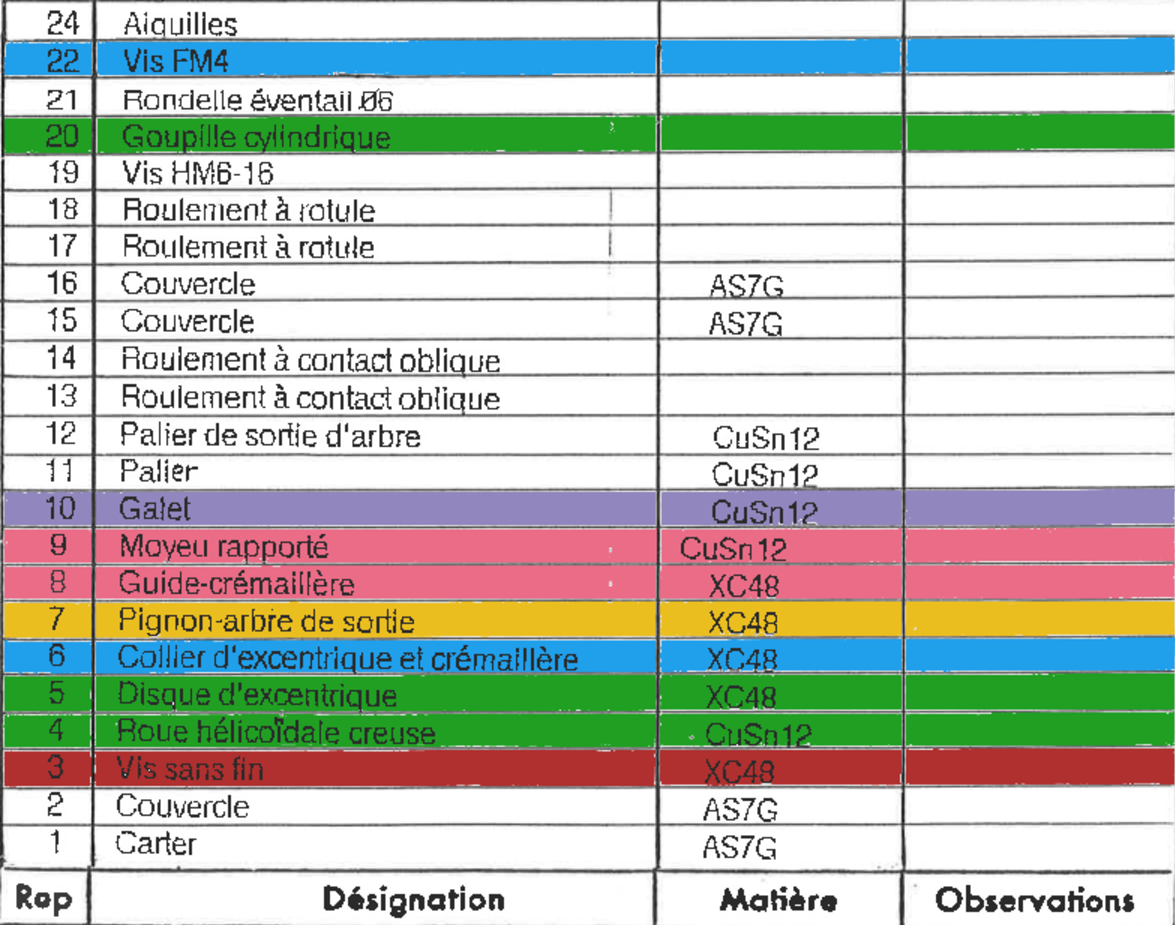
\includegraphics[width=0.7\linewidth]{img/Commande_essui_glace_nom_cor.pdf}
\end{center}

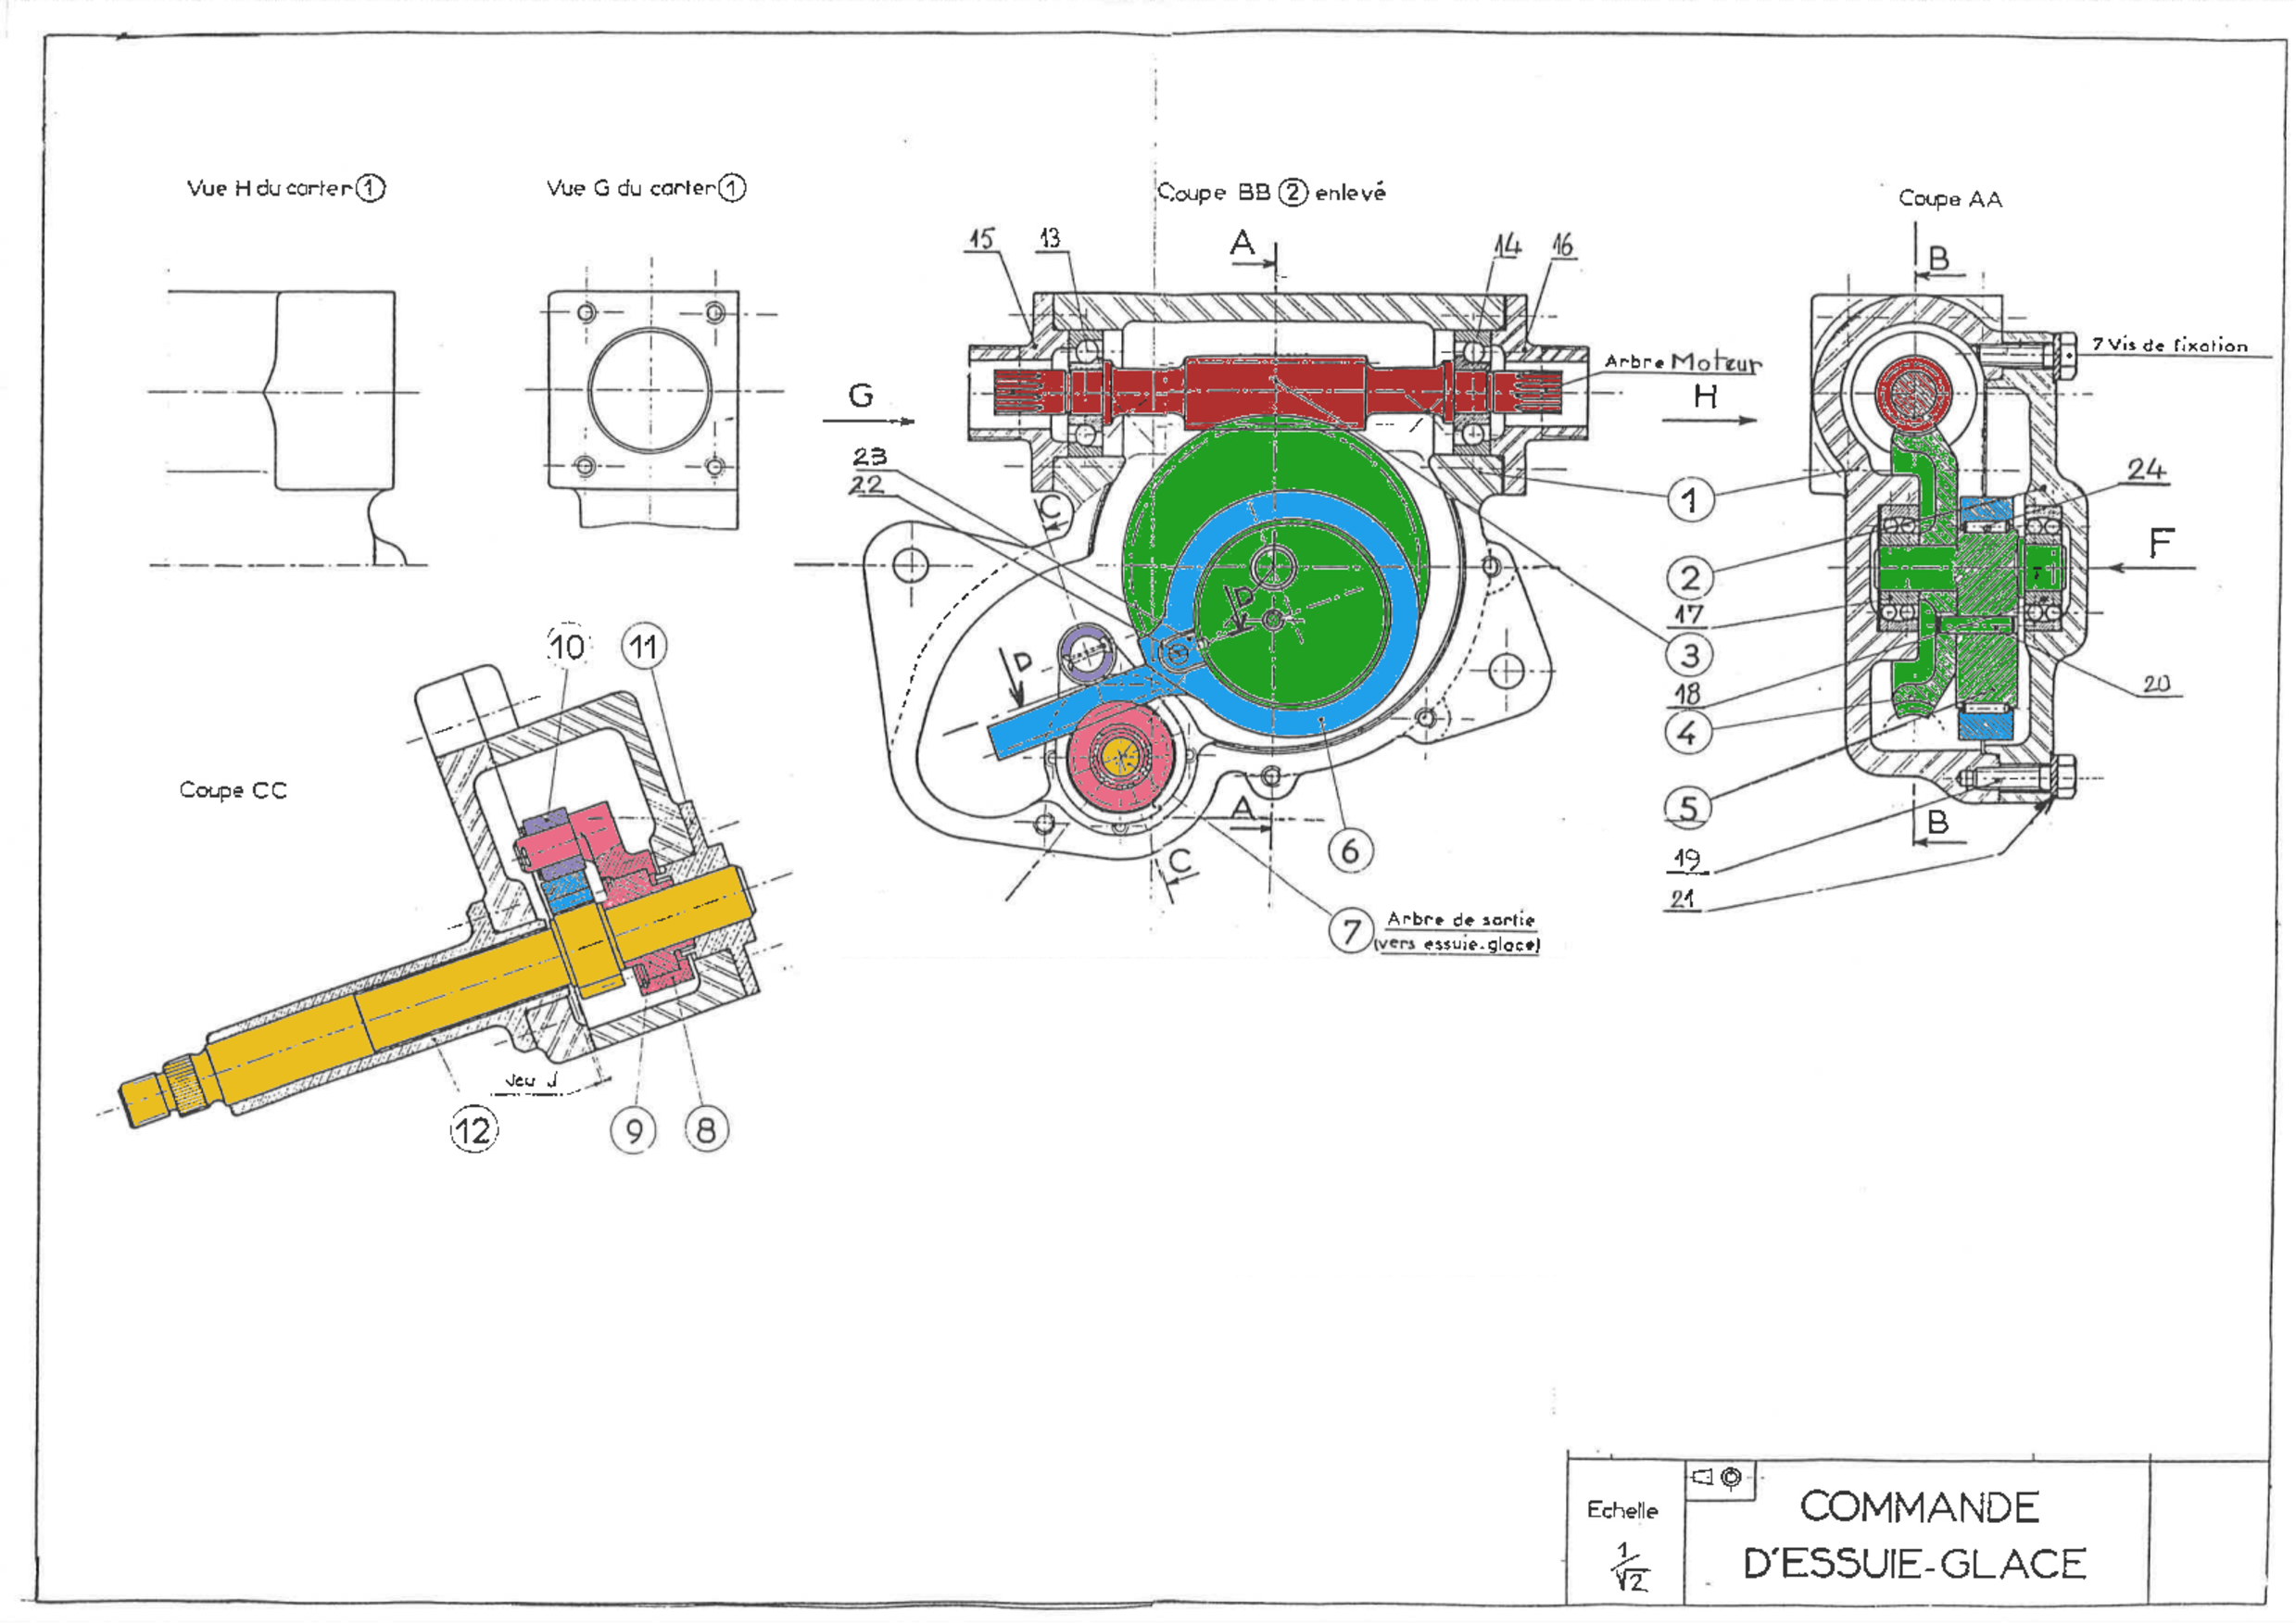
\includepdf[page=1,angle=90,offset=6mm -8mm]{img/Commande_essui_glace_dessin_cor.pdf}

\end{document}

